% Contenidos del capítulo.
% Las secciones presentadas son orientativas y no representan
% necesariamente la organización que debe tener este capítulo.

Este capítulo sitúa LocalMind-AI en el contexto de los asistentes basados en modelos de lenguaje que combinan razonamiento, recuperación de información y uso de herramientas. La primera sección examina cuatro referentes complementarios, entre los que se encuentra un mecanismo de razonamiento bajo demanda para generación de código, una aplicación de inferencia móvil y dos propuestas centradas en la planificación de herramientas y la recuperación adaptativa. En cada caso se describe su funcionamiento, su forma de despliegue y la aportación que ofrece para entender las decisiones de LocalMind-AI. La comparación no pretende establecer un orden de rendimiento entre sistemas con objetivos distintos, sino identificar qué soluciones adoptan para razonar, recuperar información y actuar mediante herramientas. A continuación se evalúan las tecnologías consideradas para materializar el proyecto y justificar sus decisiones de implementación.

\section{Análisis de tecnologías y proyectos similares para agentes de IA locales}\label{sec:tecnologias-similares-locales}

La comparación se organiza mediante dimensiones observables y no como una clasificación de rendimiento. La Tabla~\ref{tab:comparativa-sistemas-localmind} resume dónde se ejecuta la inferencia, cómo se articula el razonamiento o la agencia, qué papel tienen las herramientas o la recuperación y cómo se presenta cada propuesta al usuario. Las diferencias en la naturaleza de las fuentes se tienen en cuenta al interpretar sus afirmaciones: Think-Anywhere se consulta como \emph{preprint} y Google AI Edge Gallery a partir de su documentación oficial de código abierto, mientras que TinyAgent y Self-RAG se apoyan en publicaciones académicas. Esta precisión metodológica no altera el propósito del análisis: comparar capacidades documentadas con la arquitectura actual de LocalMind-AI.

    {\scriptsize
        \setlength{\tabcolsep}{4pt}
        \renewcommand{\arraystretch}{1.1}
        \begin{sidewaystable}[h!tp]
            \centering
            \begin{tabularx}{\textwidth}{|p{3.8cm}|p{3.5cm}|X|X|p{4.2cm}|}
                \hline
                \textbf{Sistema}                              & \textbf{Ubicación de inferencia}              & \textbf{Mecanismo de razonamiento}            & \textbf{Herramientas}                     & \textbf{Despliegue de usuario}           \\ \hline
                Think-Anywhere \cite{jiang2026thinkanywhere}  & No evaluado                                   & Bajo demanda en generación de código          & No evaluado                               & Método de investigación (sin UI)         \\ \hline
                Google AI Edge \cite{google2026aiedgegallery} & Local (móvil) mediante \gls{litert}           & Habilidades de \gls{agenteia} y funciones     & Soporte experimental \gls{mcp}            & Aplicación móvil de demostración         \\ \hline
                TinyAgent \cite{erdogan2024tinyagent}         & Local en ordenador (MacBook)                  & Planificación con \gls{llmcompiler}           & Selección de funciones con \gls{toolrag}  & Asistente \gls{macos} específico         \\ \hline
                Self-RAG \cite{asai2024selfrag}               & No evalúa cliente móvil (servidor)            & Tokens de \gls{reflexion} (recuperar/generar) & Recuperación adaptativa de pasajes        & Marco de investigación (sin UI)          \\ \hline
                LocalMind-AI                                  & Local (anfitrión) vía \gls{ollama}/\gls{omlx} & Flujo estructurado \gls{cot}-\gls{rag}        & Servidor \gls{mcp} local y \gls{chromadb} & Cliente web \gls{reactnative}/\gls{expo} \\ \hline
            \end{tabularx}
            \caption{Comparación de sistemas y métodos relacionados con LocalMind-AI.}
            \label{tab:comparativa-sistemas-localmind}
        \end{sidewaystable}
    }

\subsection{Think-Anywhere}\label{subsec:think-anywhere}

Think-Anywhere in Code Generation propone desplazar el razonamiento al momento en que la generación de código lo necesita. En vez de concentrar toda la deliberación antes de escribir, el modelo inserta bloques \texttt{<thinkanywhere>} en posiciones concretas de la secuencia generada y los elimina después para conservar código ejecutable. Con ello puede revisar una decisión local cuando aparece una incertidumbre que el plan inicial no había anticipado \parencite[pp.~1--4]{jiang2026thinkanywhere}.

El método se entrena con datos de arranque, ajuste fino con \gls{lora} y aprendizaje por refuerzo con recompensas verificables. Estas recompensas comprueban tanto la estructura de los bloques de razonamiento como la corrección ejecutable del código. Los experimentos se realizan con tareas de programación y modelos de la familia Qwen2.5-Coder, por lo que su aportación principal es un mecanismo para decidir cuándo razonar durante la generación \parencite[pp.~5--10]{jiang2026thinkanywhere}.

La Figura~\ref{fig:think-anywhere-razonamiento} reúne el diagrama conceptual conservado y dos capturas de la propuesta, donde la primera muestra la descomposición entre razonamiento previo y generación, la segunda ilustra la intervención localizada ante un error durante la codificación.

\begin{figure}[h!tp]
    \centering
    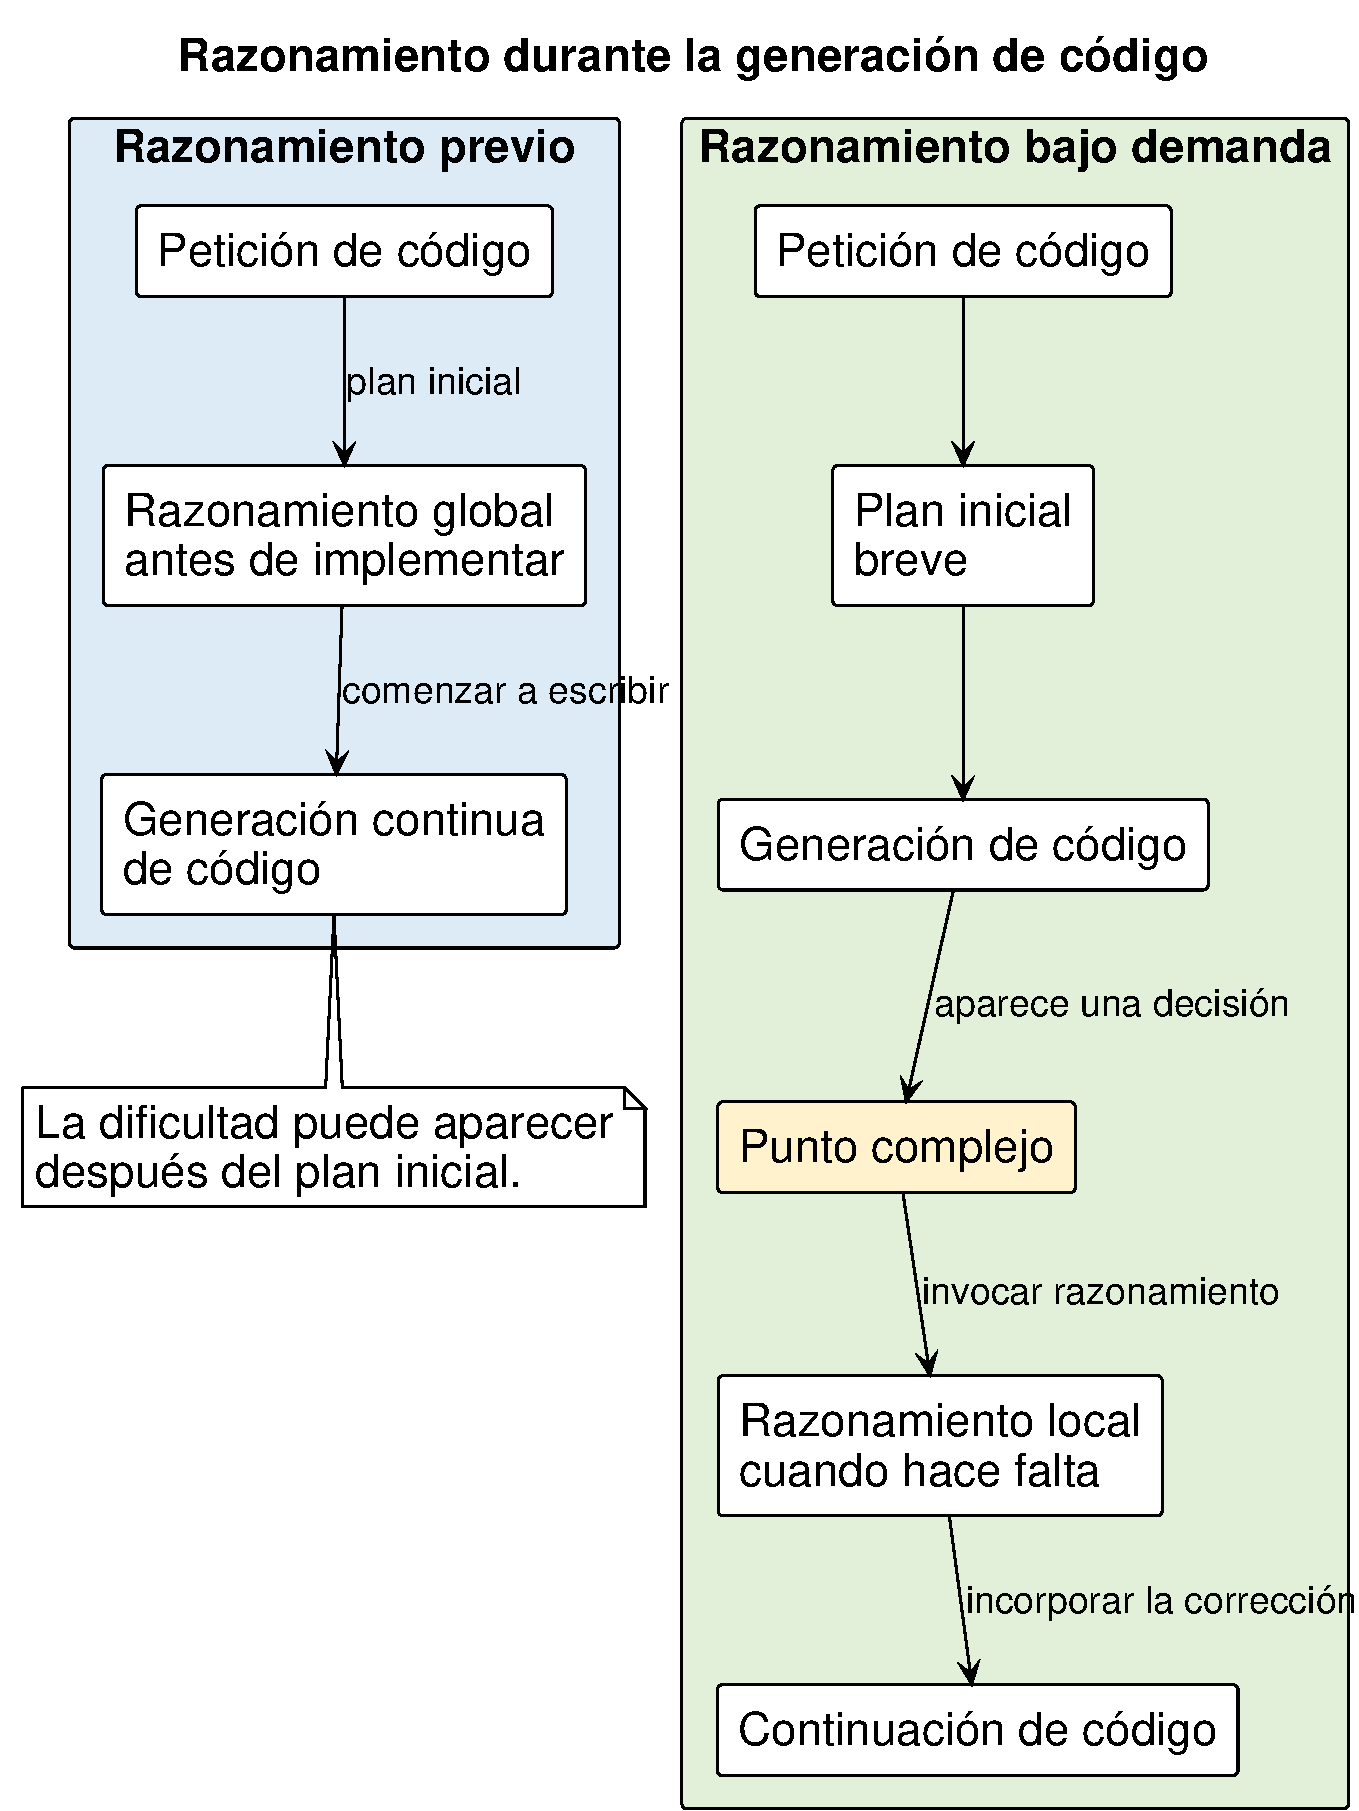
\includegraphics[width=0.48\textwidth]{figs/think-anywhere-razonamiento.pdf}\par\medskip
    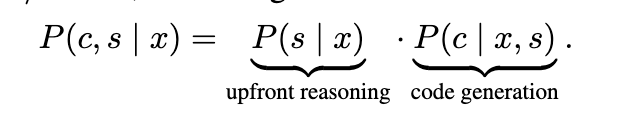
\includegraphics[width=0.65\textwidth]{figs/paper1.1.png}\par\medskip
    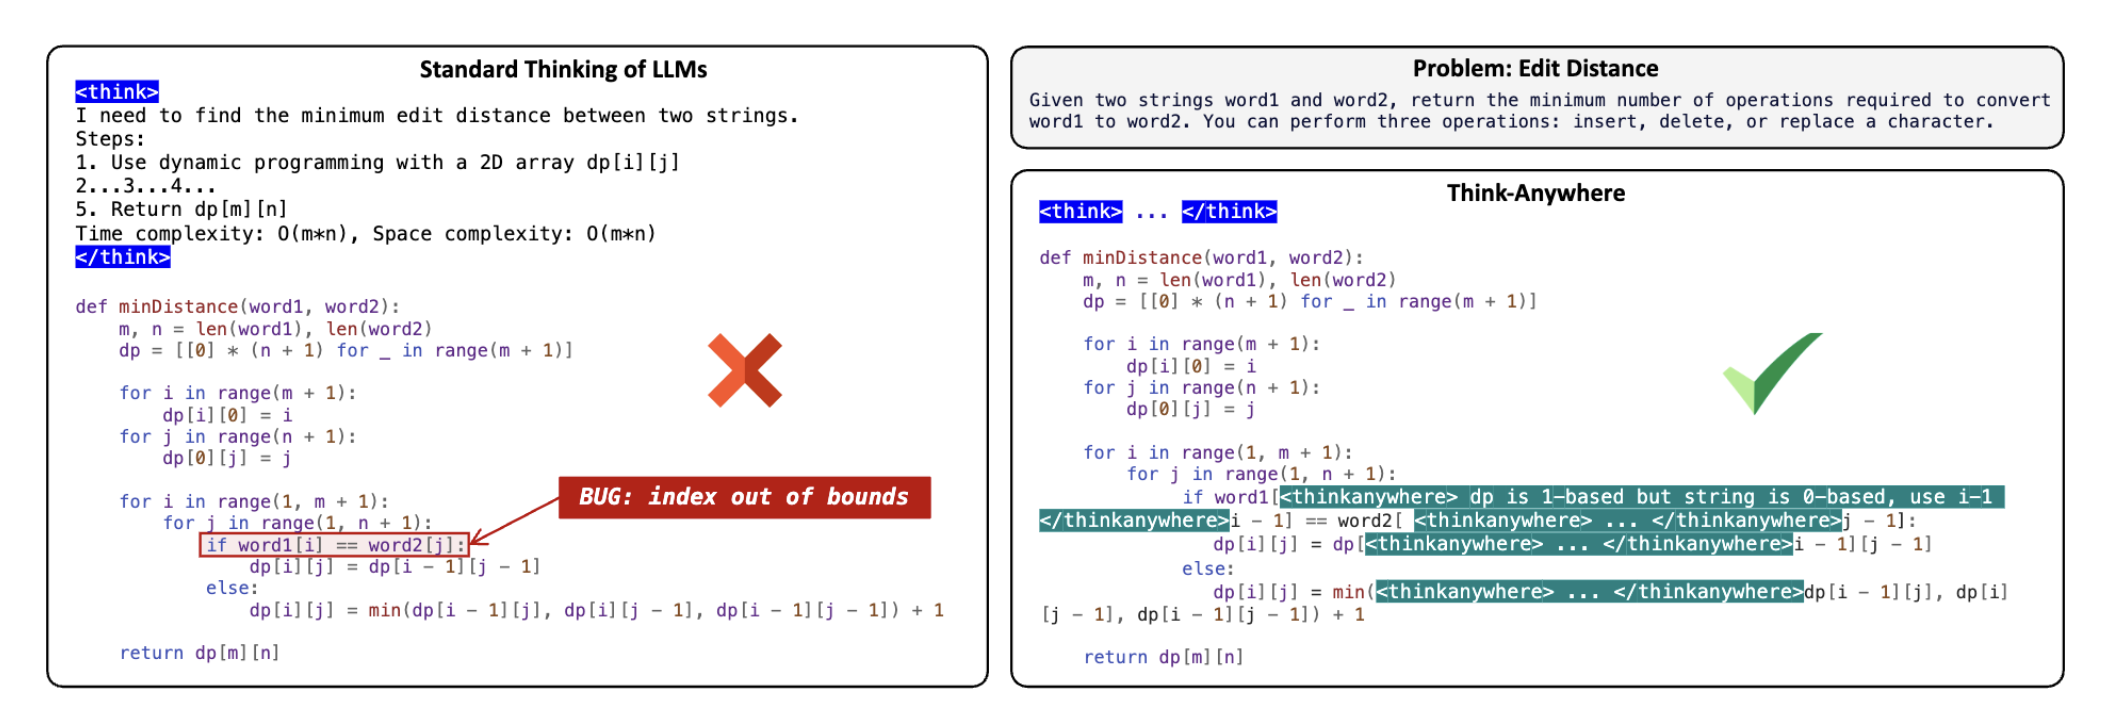
\includegraphics[width=0.92\textwidth]{figs/paper1.2.png}
    \caption[Razonamiento bajo demanda en Think-Anywhere]{Razonamiento bajo demanda en Think-Anywhere. Arriba, diagrama conceptual del artículo y abajo las capturas de la formulación y del ejemplo de generación de código de Jiang et al. \parencite[pp.~1--4]{jiang2026thinkanywhere}}
    \label{fig:think-anywhere-razonamiento}
\end{figure}

Frente a este enfoque, LocalMind-AI usa un flujo \gls{cot}-\gls{rag} guiado por instrucciones, con búsqueda en una base vectorial y herramientas expuestas por un servidor \gls{mcp}, dentro de una arquitectura local en la que el agente y el cliente web se ejecutan en contenedores separados. Think-Anywhere no persigue integrar esos componentes ni ofrecer una interfaz de usuario, por lo que su valor para LocalMind-AI está en señalar una posible evolución: decidir de forma adaptativa cuándo ampliar el razonamiento dentro de una tarea, en lugar de aplicar siempre la misma pauta de deliberación \parencite[pp.~2--6]{jiang2026thinkanywhere}.

\subsection{Google AI Edge Gallery}\label{subsec:ai-edge-gallery}

Google AI Edge Gallery es una aplicación móvil de demostración para descargar, administrar y ejecutar modelos de lenguaje en el propio dispositivo mediante \gls{litert}-LM. Permite seleccionar los backends de \gls{cpu}, \gls{gpu} o \gls{npu}, probar modelos y observar sus prestaciones desde la aplicación \cite{google2026aiedgegallery}. Además, incorpora \emph{Agent Skills}, \gls{funciontool} y soporte experimental para \gls{mcp}, de modo que las habilidades y los esquemas de herramientas se añaden al contexto de la conversación y las acciones requieren autorización del usuario \cite{google2026aiedgegallery}.

Las capturas de la Figura~\ref{fig:ai-edge-gallery-capturas} muestran la gestión de modelos, la conversación con un modelo local y la configuración de un servidor \gls{mcp}. La inferencia base se sitúa en el cliente móvil, aunque la integración de servidores remotos depende de HTTP y no permite utilizar directamente el transporte \texttt{stdio} habitual de escritorio \cite{google2026aiedgegallery}.

\begin{figure}[h!tp]
    \centering
    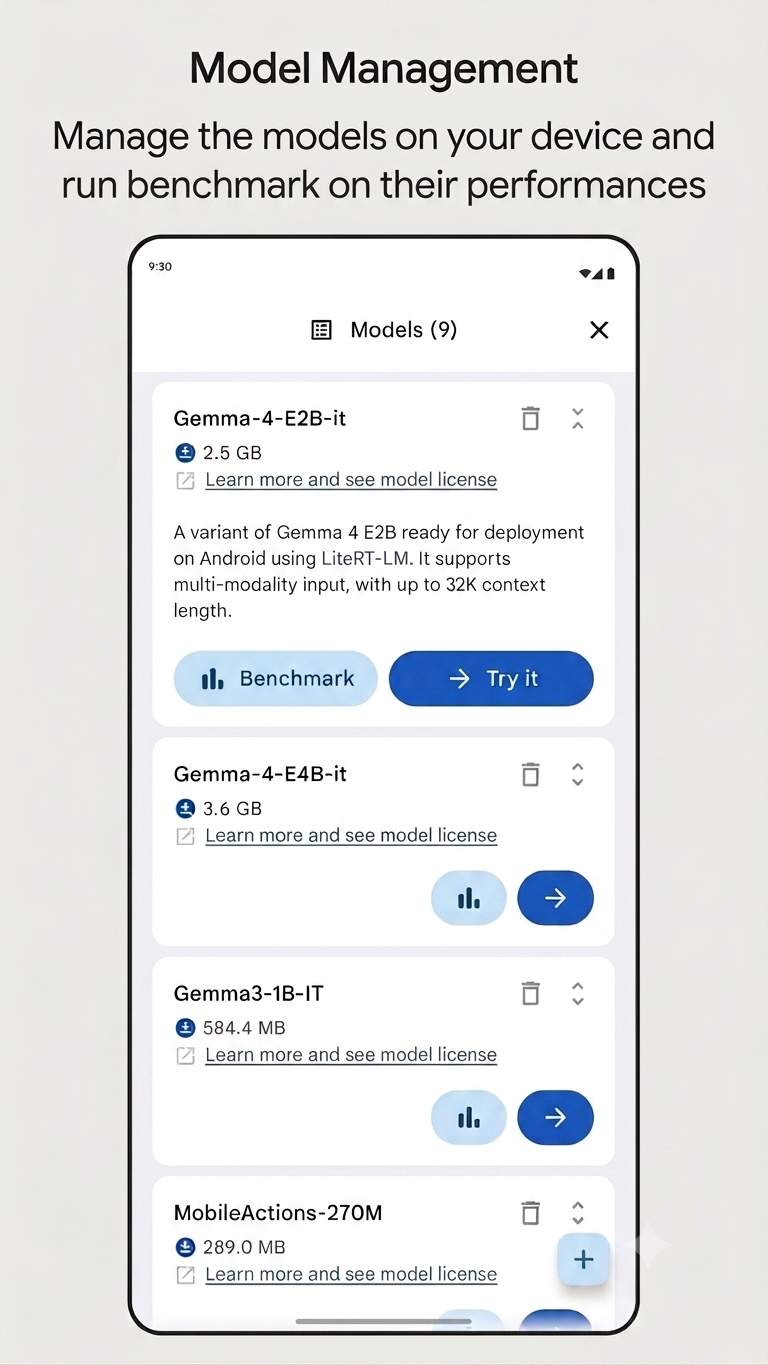
\includegraphics[height=0.35\textheight,keepaspectratio]{figs/paper2.1.png}\hfill
    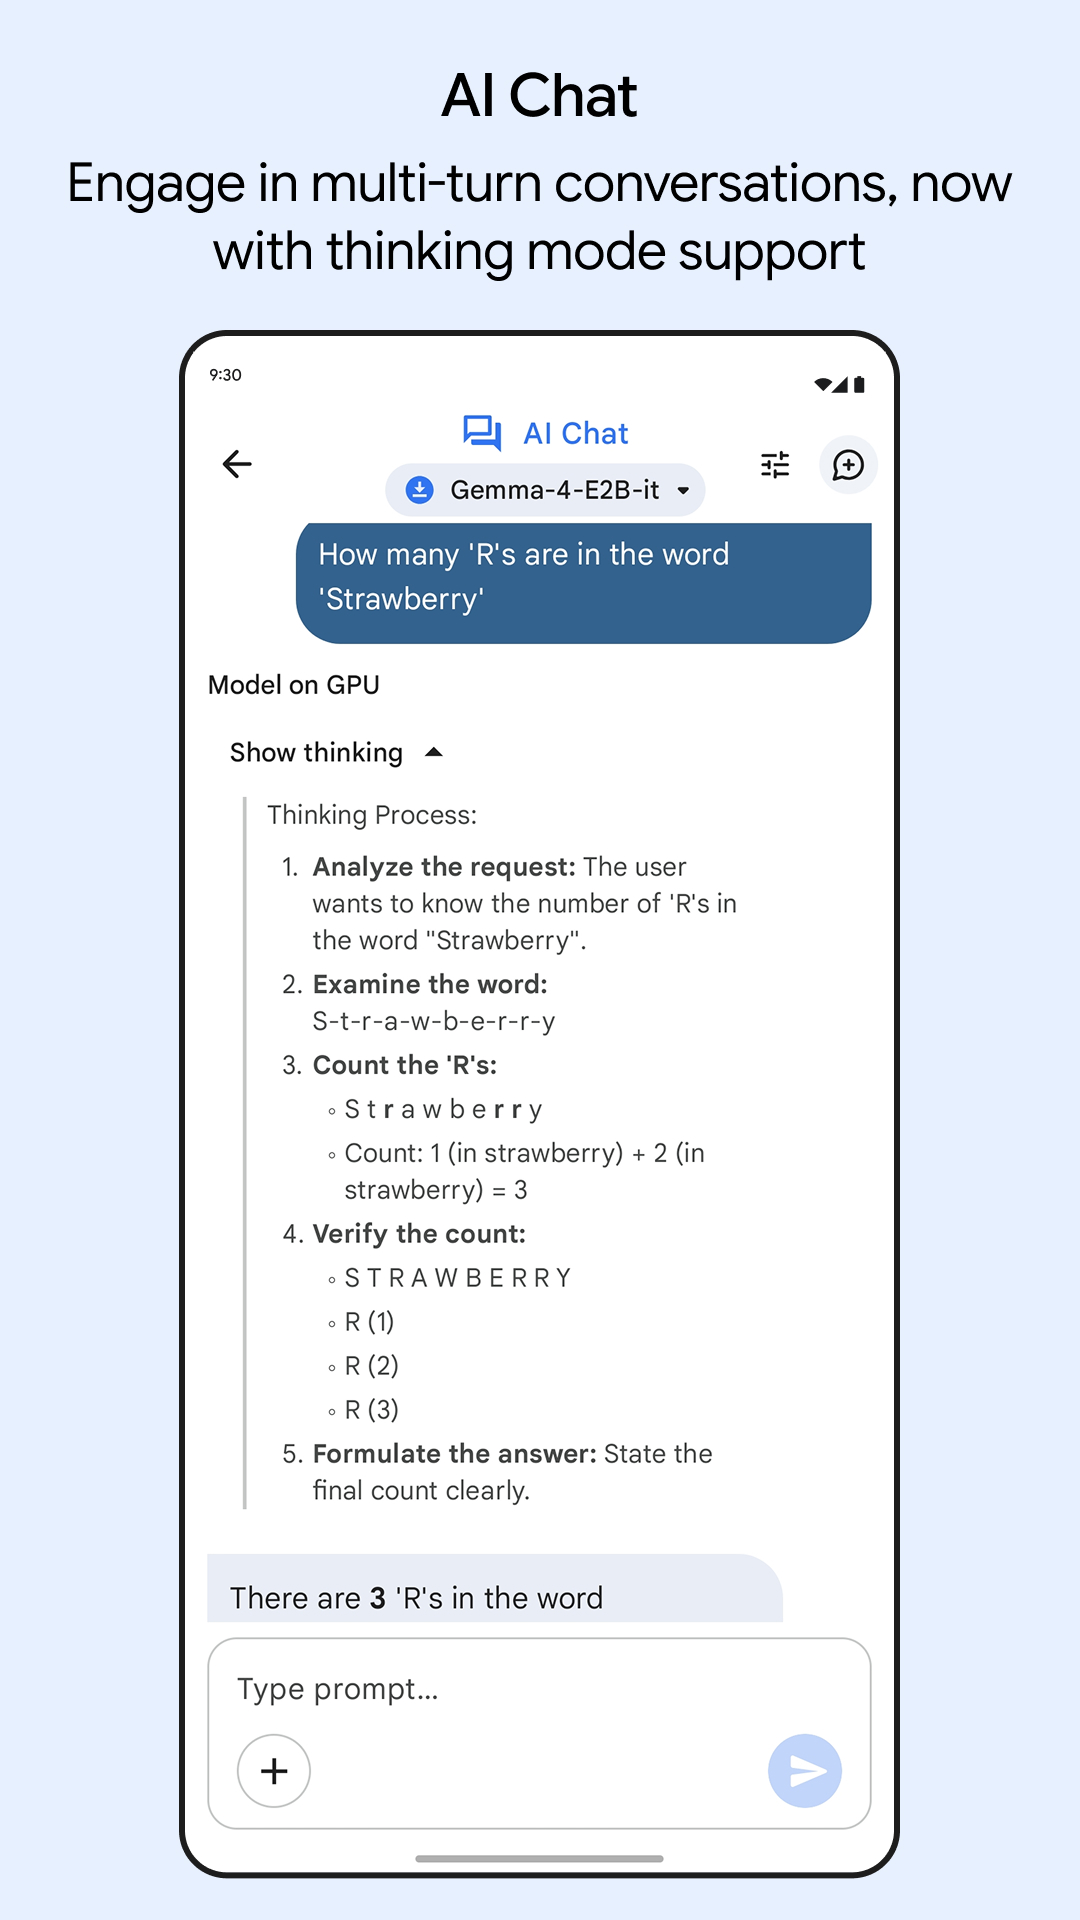
\includegraphics[height=0.35\textheight,keepaspectratio]{figs/paper2.2.jpg}\par\medskip
    
\includegraphics[height=0.33\textheight,keepaspectratio]{figs/paper2.3.png}
    \caption[Capturas de Google AI Edge Gallery]{Capturas de Google AI Edge Gallery con gestión de modelos, conversación local y administración de servidores \gls{mcp}. \cite{google2026aiedgegallery}}
    \label{fig:ai-edge-gallery-capturas}
\end{figure}

La comparación con LocalMind-AI destaca una decisión arquitectónica distinta. Edge Gallery ejecuta el modelo en el dispositivo cliente, mientras que LocalMind-AI consulta \gls{ollama} u \gls{omlx} en el anfitrión desde el contenedor del agente y entrega su aplicación \gls{reactnative} desde un segundo contenedor dedicado al cliente web. Ambos integran herramientas, pero LocalMind-AI añade un servidor \gls{mcp} propio y recuperación documental en \gls{chromadb}. Edge Gallery ofrece, por tanto, una referencia práctica sobre inferencia móvil y permisos de herramientas, mientras que LocalMind-AI prioriza la coordinación local entre modelo, recuperación y servicios.

\subsection{TinyAgent}\label{subsec:tinyagent}

TinyAgent es una demostración académica publicada en \gls{emnlp} 2024 que aborda la \gls{funciontool} en el borde mediante \glspl{agenteia} específicos de tarea. El trabajo presenta variantes de 1,1 y 7 mil millones de parámetros y utiliza \gls{llmcompiler} para obtener planes de funciones, el plan resultante expresa las dependencias entre invocaciones antes de ejecutar las herramientas \parencite[pp.~80--84]{erdogan2024tinyagent}. La contribución no consiste en una interfaz generalista, sino en articular \gls{planeacion}, selección de herramientas y ejecución para un asistente \gls{macos} con un conjunto de funciones definido \parencite[pp.~82--84]{erdogan2024tinyagent}.

Para limitar el contexto que recibe el modelo, \gls{toolrag} recupera las descripciones y los ejemplos de las herramientas pertinentes para cada solicitud. El artículo también evalúa cuantización a 4 bits como parte de su estrategia de despliegue y mide el éxito de los planes de funciones bajo las condiciones de su demostración \parencite[pp.~84--88]{erdogan2024tinyagent}. Estos resultados respaldan la discusión sobre agentes eficientes y selección de herramientas, pero están ligados a tareas, herramientas y hardware concretos, no permiten trasladar sus métricas a otros asistentes.

La Figura~\ref{fig:tinyagent-arquitectura} conserva el diagrama conceptual y añade la identificación visual del proyecto. Ambas piezas sitúan el flujo desde la petición hasta la herramienta seleccionada \parencite[pp.~80--85]{erdogan2024tinyagent}.

\begin{figure}[h!tp]
    \centering
    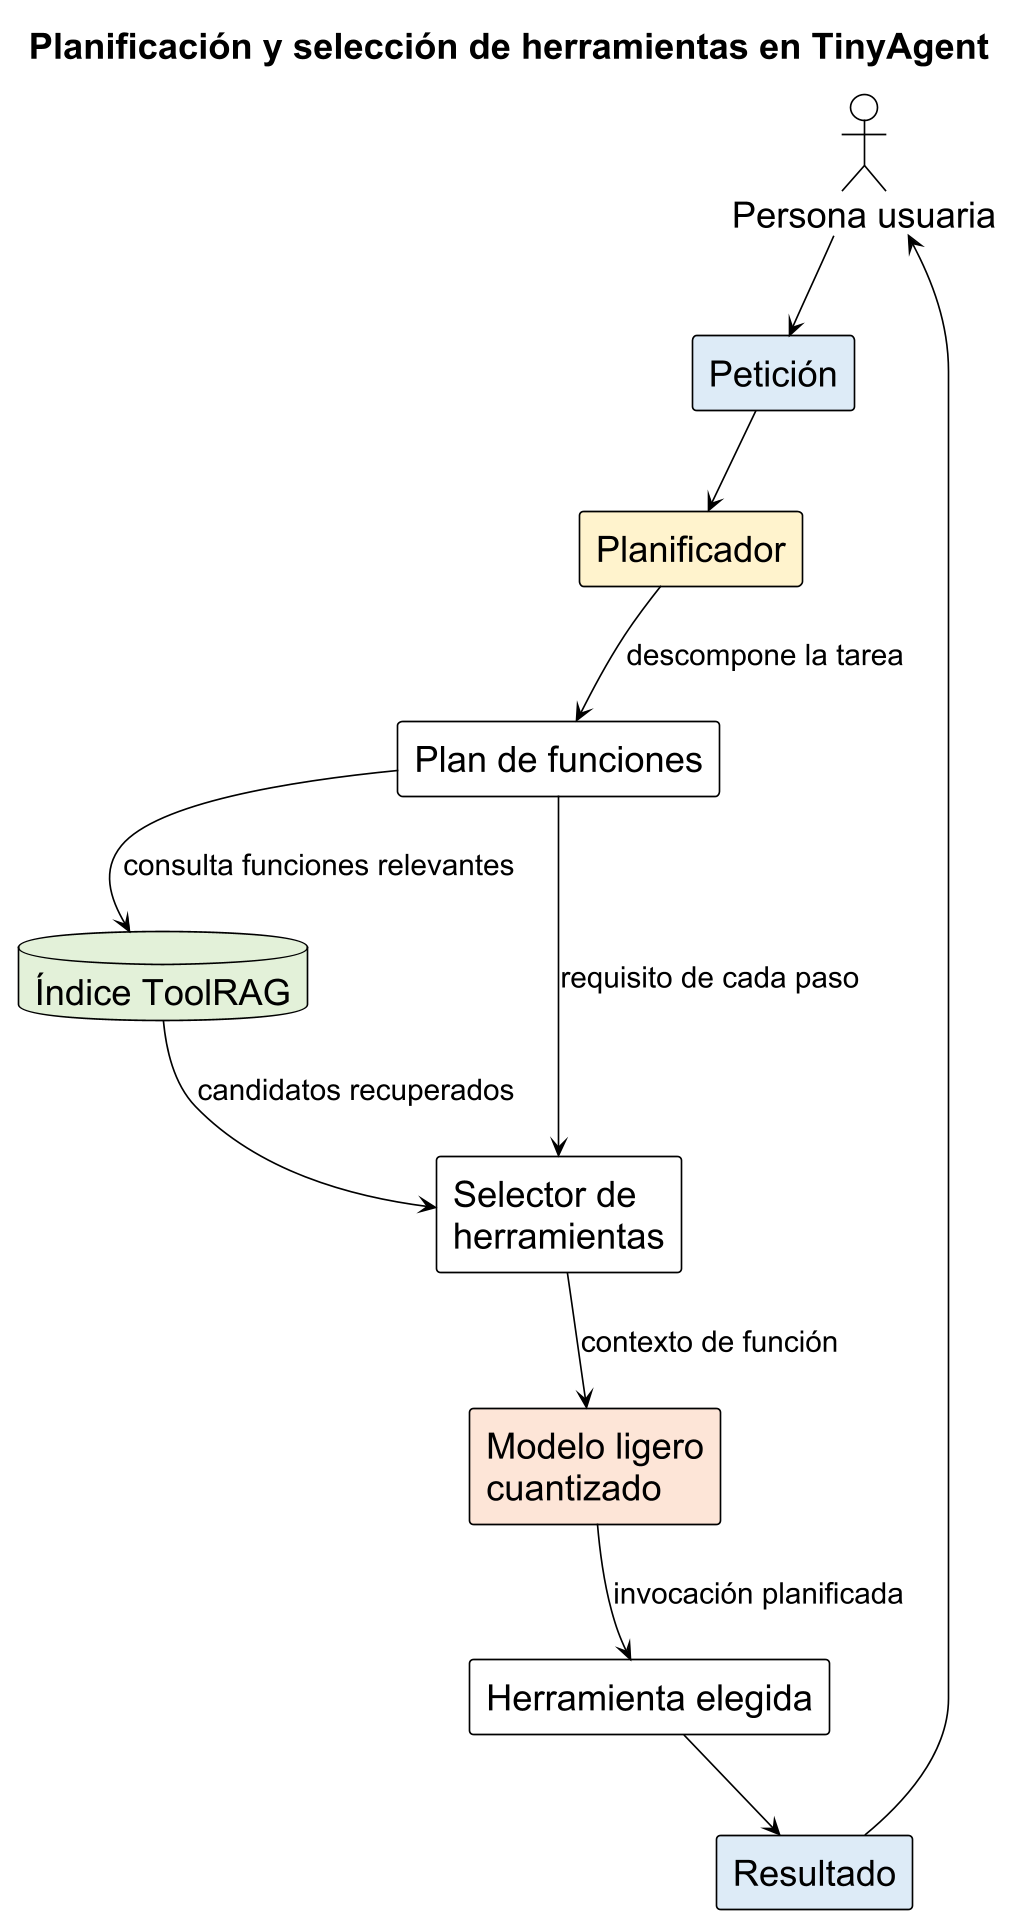
\includegraphics[width=0.46\textwidth]{figs/tinyagent-arquitectura.png}\par\medskip
    
\includegraphics[width=0.82\textwidth]{figs/paper3.1.png}
    \caption[TinyAgent y su arquitectura de planificación]{TinyAgent y su arquitectura de \gls{planeacion} y selección de herramientas. Arriba, diagrama conceptual del proyecto y abajo la identificación visual del proyecto. \parencite[pp.~80--85]{erdogan2024tinyagent}}
    \label{fig:tinyagent-arquitectura}
\end{figure}

La comparación con LocalMind-AI es parcial. TinyAgent se demuestra como asistente \gls{macos} específico de tarea y su \gls{toolrag} recupera contexto sobre herramientas, el alcance descrito no especifica integración mediante \gls{mcp} ni recuperación de una base documental general \parencite[pp.~80--88]{erdogan2024tinyagent}. Por su parte, la instantánea de LocalMind-AI documenta un flujo \gls{cot}-\gls{rag} dirigido por instrucciones, con búsqueda en \gls{chromadb}, un servidor \gls{mcp} propio y un cliente web contenido de forma independiente al agente. TinyAgent aporta así un antecedente para separar la recuperación destinada a elegir herramientas (\gls{funciontool}) de la recuperación orientada a fundamentar respuestas, sin afirmar que ambos mecanismos sean intercambiables.

\subsection{Self-RAG}\label{subsec:self-rag}

Self-RAG formula la recuperación como una decisión adaptativa durante la generación. El modelo aprende tokens de \gls{reflexion} para recuperar, generar y criticar, de forma que decide si necesita incorporar evidencia y valora la relevancia, el respaldo y la utilidad de cada resultado. Así, puede omitir la recuperación o repetirla según la evaluación interna de cada paso, frente a un flujo que recupera siempre al inicio \parencite[pp.~1--5]{asai2024selfrag}.

El artículo evalúa esta arquitectura en tareas de pregunta-respuesta, razonamiento, verificación factual y generación extensa. La Figura~\ref{fig:self-rag-captura} muestra la diferencia visual entre un flujo \gls{rag} convencional y la recuperación, generación y crítica iterativas de Self-RAG \parencite[pp.~1, 6--10]{asai2024selfrag}.

\begin{figure}[h!tp]
    \centering
    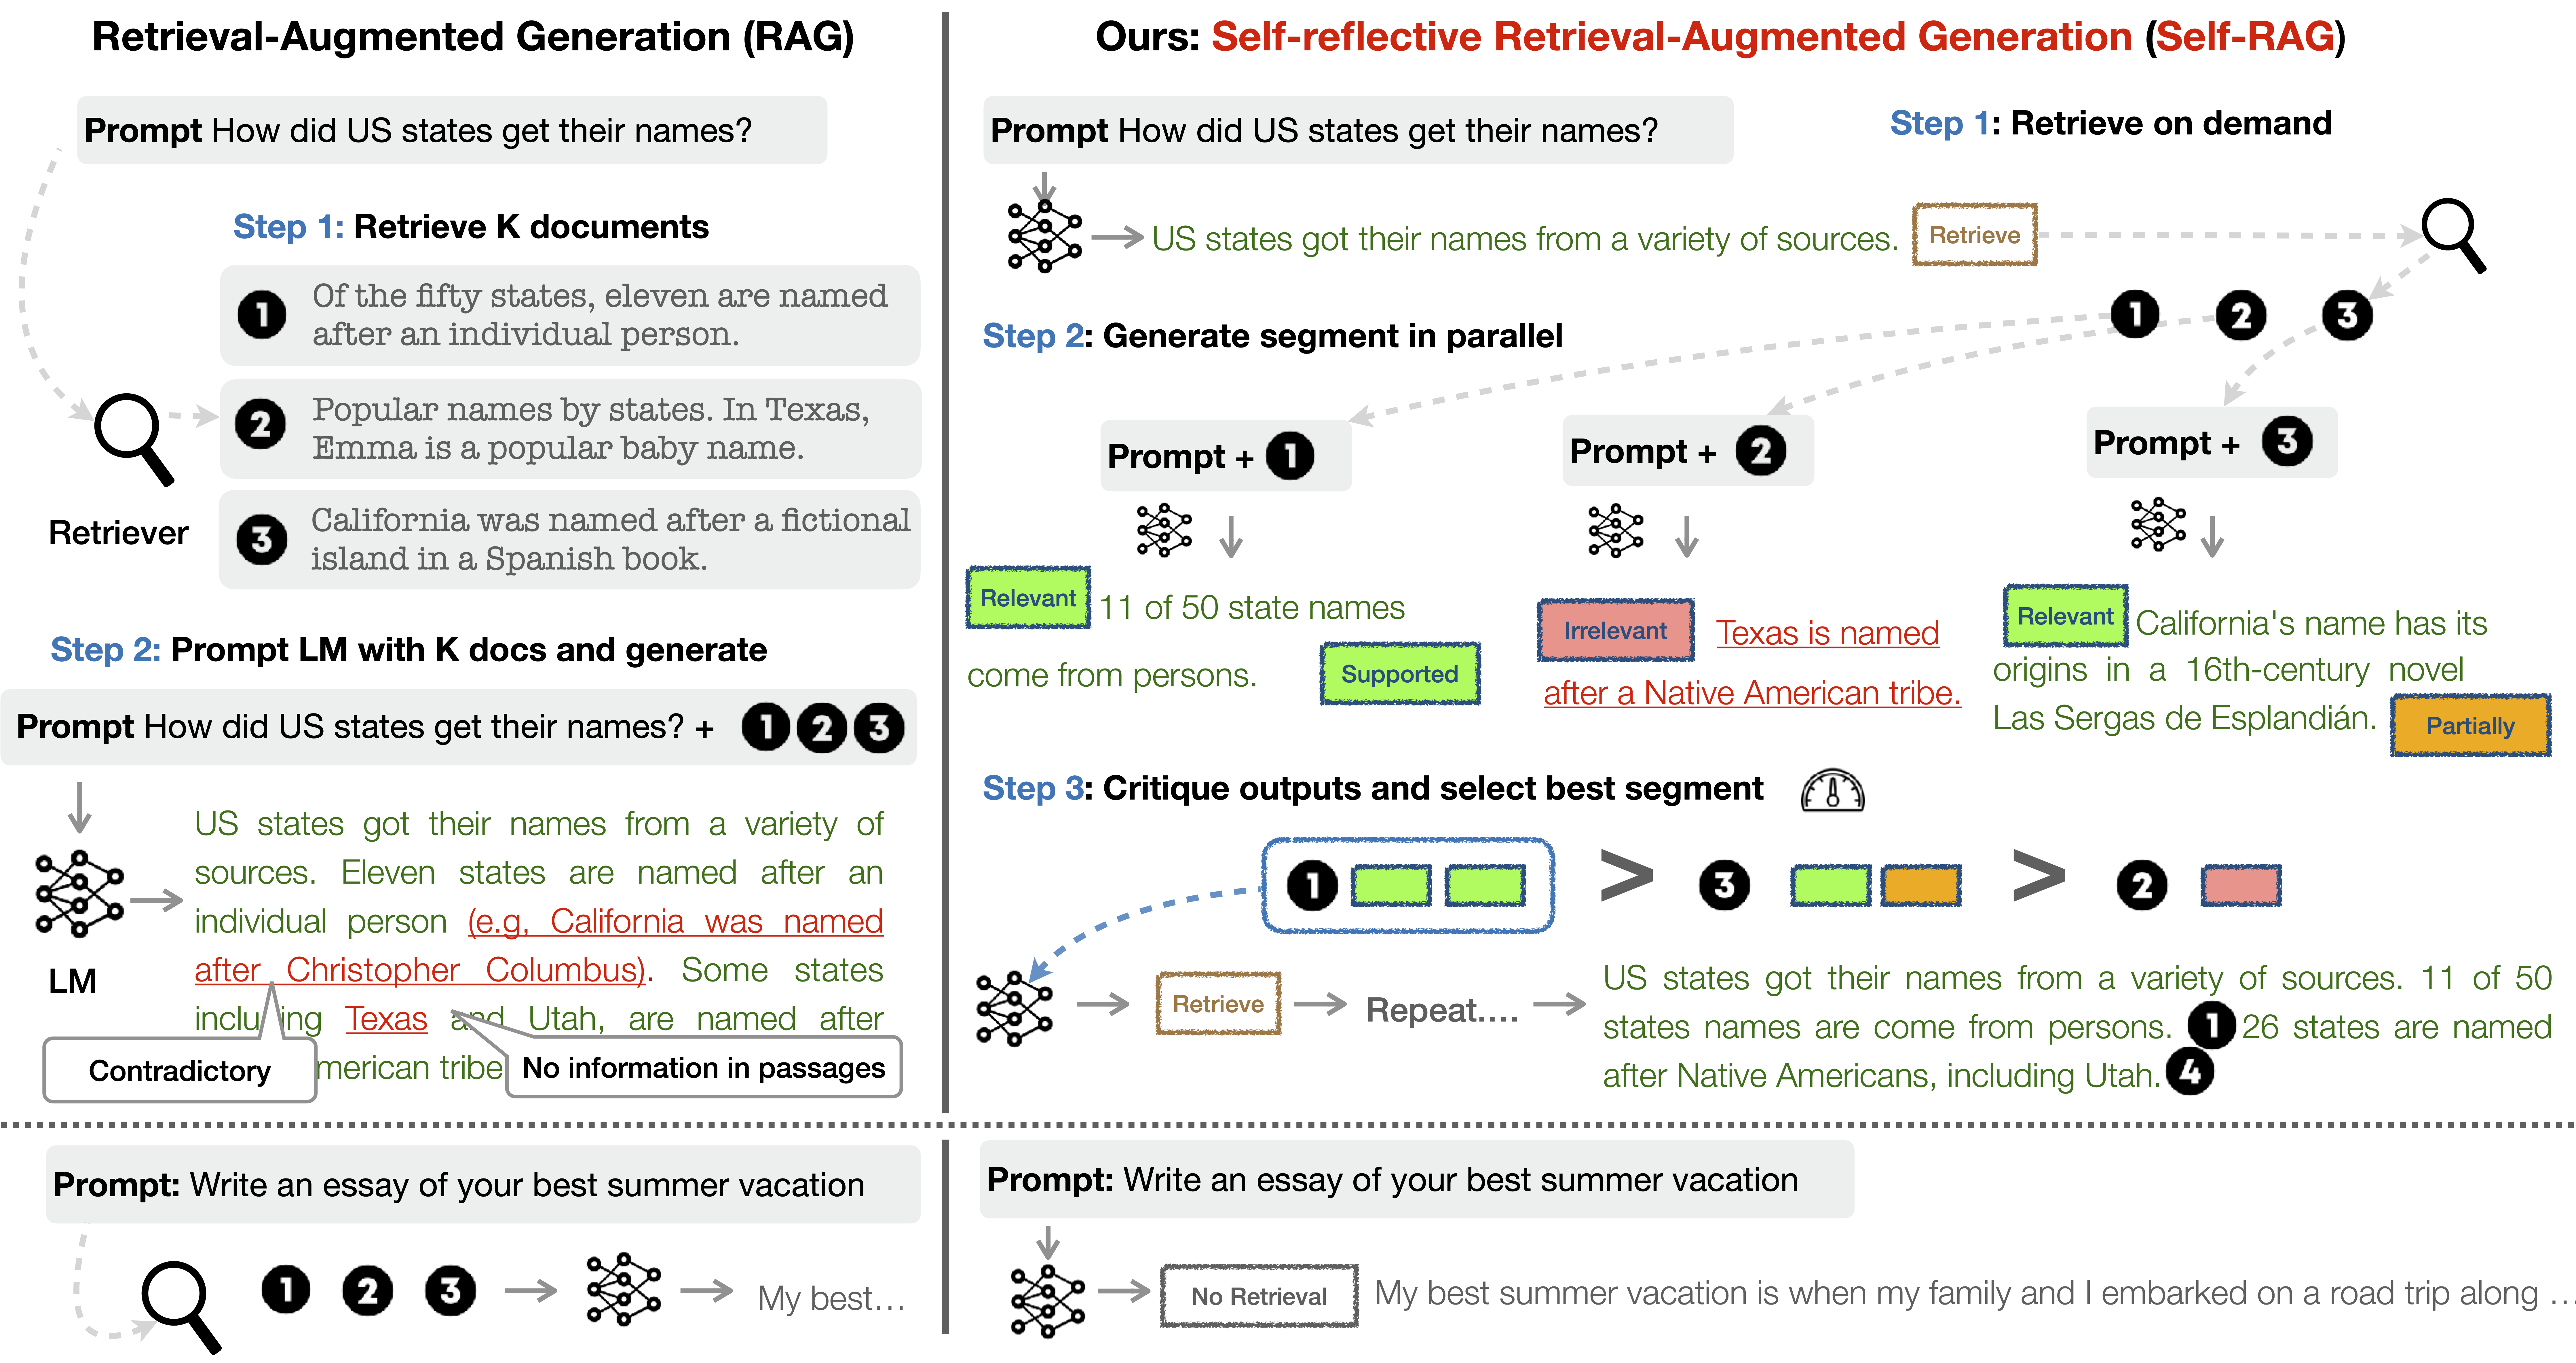
\includegraphics[width=0.95\textwidth]{figs/paper4.1.png}
    \caption[Comparación entre RAG y Self-RAG]{Comparación entre un flujo \gls{rag} convencional y la recuperación autorreflexiva de Self-RAG. \parencite[pp.~1--5]{asai2024selfrag}}
    \label{fig:self-rag-captura}
\end{figure}

La comparación con LocalMind-AI se sitúa en la coordinación entre razonamiento y recuperación. LocalMind-AI documenta un flujo \gls{cot}-\gls{rag} guiado por instrucciones, con herramientas accesibles mediante \gls{mcp} y una base \gls{chromadb}, separando además el agente y el cliente web en dos servicios contenerizados. Self-RAG integra la decisión de recuperar y la crítica en el modelo entrenado, mientras que LocalMind-AI orquesta esos componentes desde su arquitectura de aplicación. Por ello, Self-RAG sirve como referencia para valorar estrategias de recuperación adaptativa, no como una descripción de una capacidad ya implementada en LocalMind-AI \parencite[pp.~1--5]{asai2024selfrag}.

\subsection{Conclusiones}\label{subsec:conclusiones-tecnologias-similares}

Los cuatro casos examinados cubren dimensiones complementarias y no son equivalentes como productos ni como evidencia. Think-Anywhere estudia el razonamiento bajo demanda para generación de código y se mantiene en condición de \emph{preprint} sin revisión por pares \cite{jiang2026thinkanywhere}. Google AI Edge Gallery aporta evidencia oficial no académica sobre inferencia en el cliente móvil, habilidades y soporte experimental de \gls{mcp} \cite{google2026aiedgegallery}. TinyAgent demuestra \gls{planeacion} de funciones y selección de contexto de herramientas en un asistente macOS específico de tarea \cite{erdogan2024tinyagent}, Self-RAG aporta una arquitectura de investigación para decidir, recuperar, generar y criticar durante la producción de una respuesta \cite{asai2024selfrag}. Esta diversidad explica por qué una comparación controlada debe atender al alcance de cada fuente, no derivar un orden de rendimiento entre propuestas heterogéneas.

LocalMind-AI se diferencia por la combinación documentada de un modelo servido por \gls{ollama} o \gls{omlx} en un host local, un cliente \gls{reactnative}/\gls{expo} y un agente desplegados en contenedores independientes, servidores \gls{mcp} iniciados como subprocesos y recuperación sobre \gls{chromadb} dentro de un flujo \gls{cot}-\gls{rag} dirigido por instrucciones. Esa combinación permite situarlo entre los referentes anteriores sin prometer capacidades no implementadas, ya que la evidencia actual no acredita inferencia directamente en el cliente como Edge Gallery, \gls{planeacion} entrenada de funciones como TinyAgent, ni autorreflexión adaptativa entrenada como Self-RAG \cite{google2026aiedgegallery,erdogan2024tinyagent,asai2024selfrag}. Del mismo modo, Think-Anywhere informa una posible línea de razonamiento adaptativo, pero no valida el despliegue, la recuperación documental ni las herramientas de LocalMind-AI \cite{jiang2026thinkanywhere}. La aportación diferenciada del proyecto es, por tanto, la integración observada de esos componentes en un asistente de ámbito local, cuya evaluación tecnológica se desarrolla en la sección siguiente.

\section{Evaluación de tecnologías para el desarrollo del TFM}\label{sec:evaluacion-tecnologias}

La evaluación de tecnologías se organiza en tres bloques principales, correspondientes a hardware, infraestructura y software. Esta división permite analizar cada herramienta según su función real sin mezclar conceptos. El criterio central del proyecto es el enfoque \emph{local-first} de LocalMind-AI, por el que los modelos de lenguaje, la base de datos vectorial y la memoria de trabajo deben ejecutarse y almacenarse en el equipo del usuario. A continuación, se detallan las alternativas consideradas en cada apartado y se justifica la elección final.

\subsection{Hardware}\label{subsec:hardware-localmind}

\subsubsection{Ordenadores de desarrollo y validación}

Para comprobar el rendimiento del sistema se han evaluado tres portátiles con características distintas. El modelo HP OMEN actúa como referencia histórica de recursos limitados, mientras que los equipos de MSI y Apple permiten validar la solución en los dos entornos previstos, que corresponden a \gls{windows} con tarjeta gráfica dedicada NVIDIA y \gls{macos} con chips Apple Silicon.

\paragraph{OMEN by HP 15-ce033ns.}
Este equipo sirve como referencia histórica y cuenta con las siguientes especificaciones \cite{hp2017omen15ce033ns}.
\begin{itemize}[leftmargin=*,nosep]
    \item \textbf{Procesador.} Intel Core i7-7700HQ (4 núcleos, 2,8~GHz base y hasta 3,8~GHz turbo).
    \item \textbf{Memoria \gls{ram}.} 12~GB de SDRAM DDR4-2400.
    \item \textbf{Tarjeta gráfica.} NVIDIA GeForce GTX 1050 con 2~GB de \gls{vram} GDDR5 dedicada.
    \item \textbf{Almacenamiento.} Disco duro SATA de 1~TB a 7200~rpm.
    \item \textbf{Función en el proyecto.} Referencia de hardware antiguo, no se utiliza como equipo objetivo de pruebas.
\end{itemize}
Los 2~GB de \gls{vram} y la antigüedad del procesador limitan tanto el tamaño de los modelos como la ejecución simultánea del agente, la interfaz y el motor de inferencia. Por ello, se descarta para las pruebas principales.

\paragraph{MSI Pulse GL66 12UEK-085ES.}
Es un portátil de rendimiento medio-alto que venía de fábrica con 16~GB de memoria \cite{MSIPulseGL66}. Para este TFM se utiliza con la siguiente configuración.
\begin{itemize}[leftmargin=*,nosep]
    \item \textbf{Procesador.} Intel Core i7-12700H (14 núcleos, 20 hilos, de 2,3 a 4,7~GHz).
    \item \textbf{Memoria \gls{ram}.} Ampliada por el autor a 32~GB DDR4-3200 en dos módulos de 16~GB.
    \item \textbf{Tarjeta gráfica.} NVIDIA GeForce RTX 3060 con 6~GB de \gls{vram} GDDR6 dedicada.
    \item \textbf{Almacenamiento.} SSD NVMe PCIe de 1~TB.
    \item \textbf{Función en el proyecto.} Equipo principal de validación para \gls{windows} y \gls{linux}, con aceleración \gls{cuda} para la inferencia nativa y \gls{docker} para los componentes de aplicación.
\end{itemize}
La ampliación a 32~GB de \gls{ram} realizada por el autor permite ejecutar al mismo tiempo los contenedores de la aplicación y los modelos cuantizados en el anfitrión, aunque los 6~GB de \gls{vram} limitan el tamaño máximo de los modelos que se pueden cargar en la \gls{gpu}.

\paragraph{MacBook Air M4.}
Es el equipo elegido para validar el entorno \gls{macos} con Apple Silicon \cite{apple2025macbookair}.
\begin{itemize}[leftmargin=*,nosep]
    \item \textbf{Procesador.} Chip Apple M4 con \gls{cpu} de 10 núcleos.
    \item \textbf{Memoria \gls{ram}.} 16~GB de memoria unificada compartida entre \gls{cpu}, \gls{gpu} y sistema.
    \item \textbf{Aceleración hardware.} \Gls{gpu} integrada de 10 núcleos y Neural Engine de 16 núcleos mediante el entorno \gls{mlx}.
    \item \textbf{Almacenamiento.} SSD de 512~GB.
    \item \textbf{Función en el proyecto.} Redacción de la memoria y equipo de validación para \gls{macos} con \gls{omlx} y \gls{mlx}.
\end{itemize}
La arquitectura de memoria unificada evita copiar datos entre la \gls{ram} y la \gls{vram}, reduciendo la latencia. Sin embargo, al compartir esos 16~GB con el sistema operativo y el navegador, la cuantización del modelo resulta clave para no agotar la memoria.

\textbf{Decisión.} Se descarta el HP OMEN como entorno de pruebas. La validación de LocalMind-AI se realiza de forma dual en el MSI Pulse GL66 y en el MacBook Air M4, cubriendo así dos arquitecturas de aceleración muy diferentes (NVIDIA \gls{cuda} y Apple Silicon).

\subsection{Infraestructura, virtualización y despliegue}\label{subsec:contenedores-localmind}

\subsubsection{Sistemas operativos anfitriones}

LocalMind-AI está diseñado para funcionar en \gls{windows} y \gls{macos}, manteniendo compatibilidad con \gls{linux} en equipos donde estén disponibles \gls{docker}, \gls{python} y el motor de inferencia elegido. El proyecto no requiere instalar ni gestionar explícitamente \gls{wsl2}; en Windows, Docker Desktop puede abstraer internamente esta capa sin incorporarla al flujo de configuración de LocalMind-AI. De este modo, en \gls{macos} la inferencia se apoya en \gls{mlx}, mientras que en \gls{windows} o \gls{linux} se utiliza \gls{ollama} con aceleración NVIDIA \cite{ollama2024,omlx2026}.

\subsubsection{Tecnologías de gestión de contenedores}

Para la virtualización ligera se dispone de diversas alternativas con filosofías de arquitectura diferenciadas. \Gls{docker} constituye el formato estándar y el ecosistema más consolidado para definir imágenes, redes y volúmenes persistentes mediante un demonio centralizado \cite{DockerAcceleratedContainer2022}. Por su parte, \Gls{podman} ofrece una herramienta compatible con la especificación de la Open Container Initiative que opera sin demonio central (\emph{daemonless}), facilitando la ejecución en entornos restringidos o sin privilegios de administración \cite{podman2026}. Como propuesta reciente en sistemas Apple Silicon, la herramienta de código abierto \gls{containercli} de Apple (\texttt{apple/container}) proporciona una solución nativa para gestionar contenedores Linux sobre \gls{macos} utilizando directamente el marco de virtualización del sistema operativo y el hipervisor de Darwin con una huella de memoria reducida \cite{applecontainer2026}. Por último, \Gls{lxc} proporciona contenedores de sistema orientados a la virtualización completa del sistema operativo, lo que resulta más pesado y menos adecuado para aislar los microservicios discretos de LocalMind-AI \cite{lxc2026}.

En la Figura~\ref{fig:PodmanDocker} se ilustra la comparación conceptual entre la arquitectura sin demonio de Podman y el demonio central de Docker. Asimismo, en la Figura~\ref{fig:LXCDocker} se resumen las diferencias entre la virtualización de sistema propia de LXC y la virtualización de aplicación basada en Docker. Por su parte, la Figura~\ref{fig:AppleContainerDocker1} y la Figura~\ref{fig:AppleContainerDocker2} detallan la comparación estructural y de flujo de ejecución entre el entorno nativo de Apple Container CLI y la arquitectura convencional de Docker.

\begin{figure}[h!tp]
    \centering
    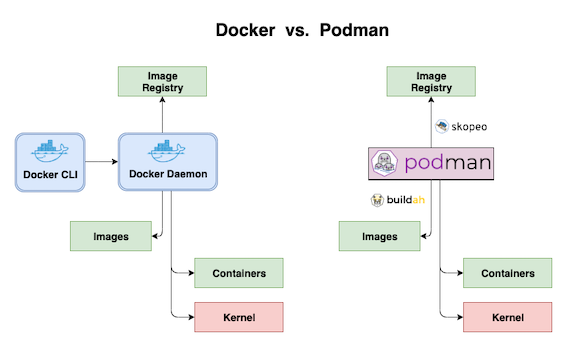
\includegraphics[width=0.78\textwidth]{figs/PodmanDocker.png}
    \caption{Comparación conceptual entre las arquitecturas de Podman y Docker.}
    \label{fig:PodmanDocker}
\end{figure}

\begin{figure}[h!tp]
    \centering
    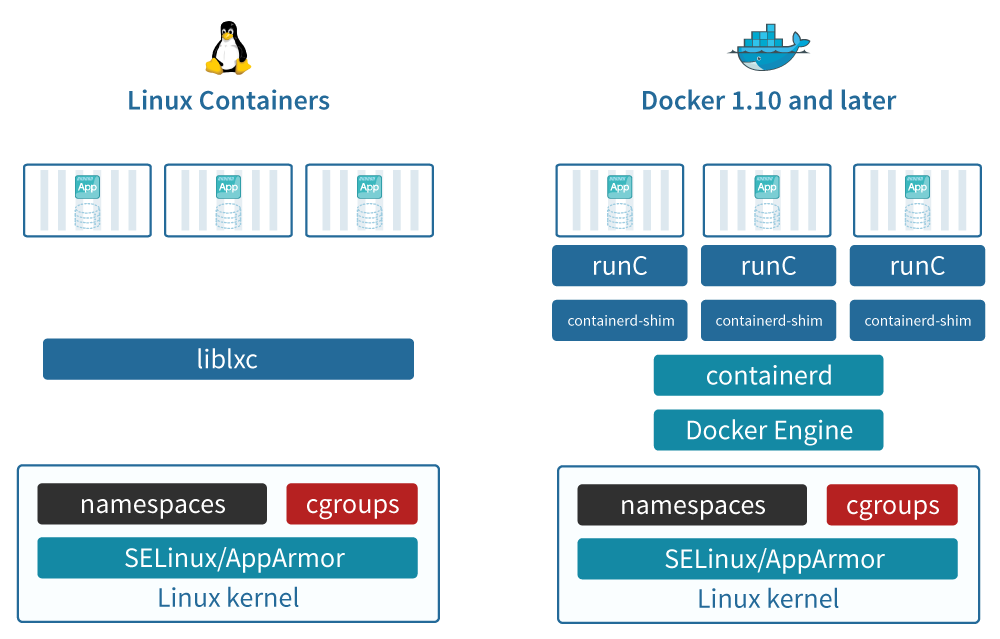
\includegraphics[width=0.78\textwidth]{figs/LXCDocker.png}
    \caption{Comparación conceptual entre los contenedores de sistema LXC y los contenedores de aplicación Docker.}
    \label{fig:LXCDocker}
\end{figure}

\begin{figure}[h!tp]
    \centering
    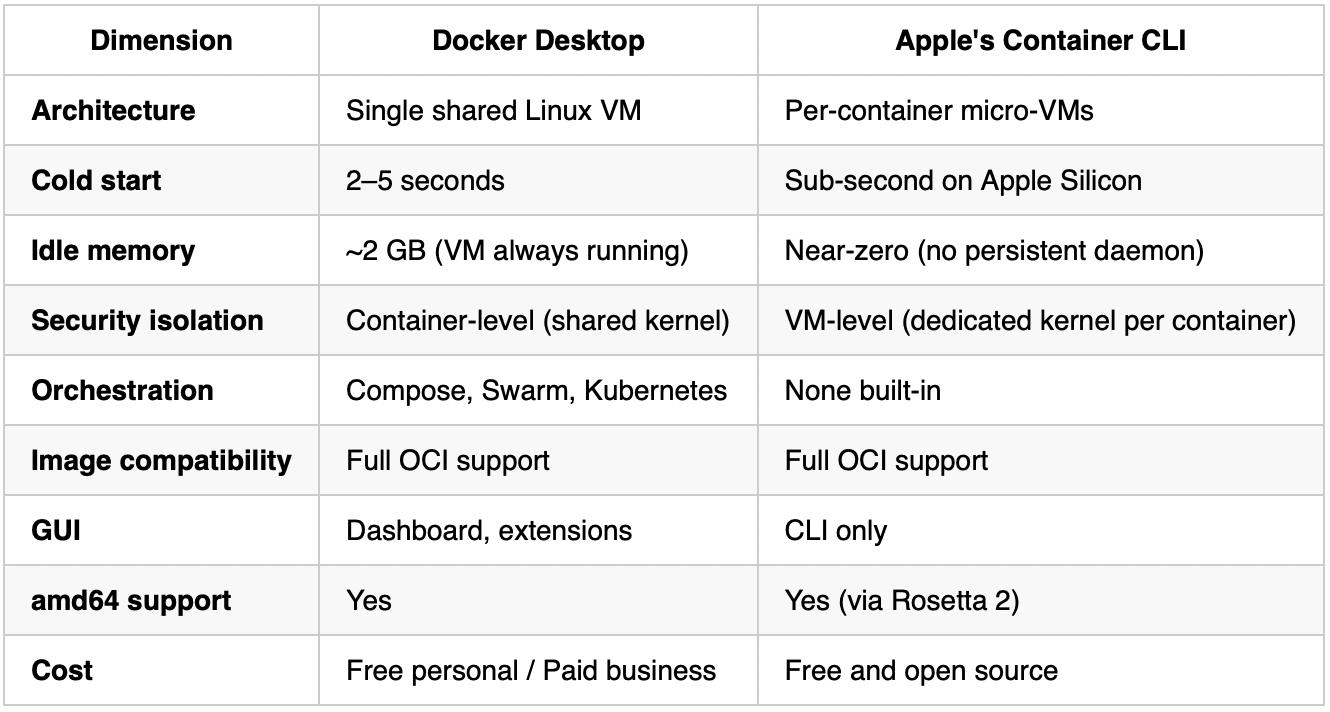
\includegraphics[width=0.78\textwidth]{figs/comp_containerVSdocker1.jpeg}
    \caption{Comparación estructural entre la arquitectura nativa de Apple Container CLI y Docker.}
    \label{fig:AppleContainerDocker1}
\end{figure}

\begin{figure}[h!tp]
    \centering
    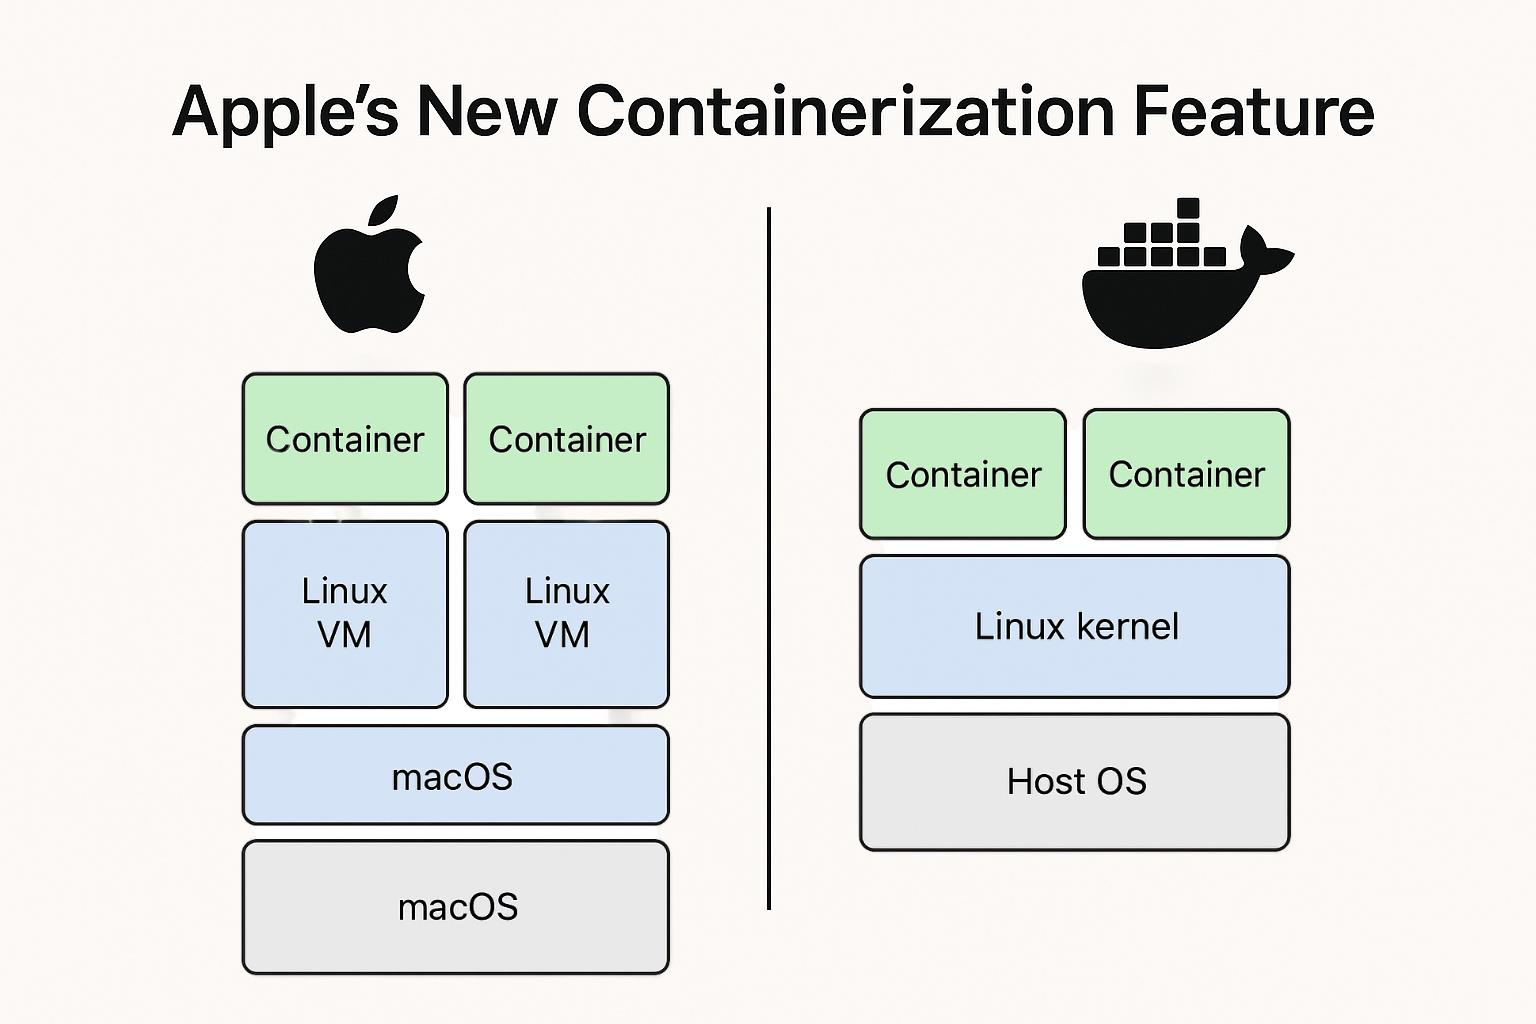
\includegraphics[width=0.78\textwidth]{figs/comp_containerVSdocker2.jpeg}
    \caption{Comparación de flujo de ejecución entre Apple Container CLI y la infraestructura de Docker.}
    \label{fig:AppleContainerDocker2}
\end{figure}

\textbf{Decisión.} Se adopta \gls{docker} como motor de ejecución principal debido a su soporte multiplataforma garantizado en \gls{windows}, \gls{macos} y \gls{linux}, su ecosistema de orquestación y su capacidad para ofrecer un entorno de validación reproducible. Las herramientas Podman y \gls{containercli} de Apple representan alternativas válidas y prometedoras para entornos sin demonio o específicos de \gls{macos}, si bien la solución basada en Docker permite mantener una especificación unificada sin introducir dependencias exclusivas de una plataforma concreta.

\subsubsection{Orquestación del despliegue con Docker Compose}

Desplegar manualmente los contenedores exige gestionar a mano los puertos, los volúmenes de datos y las variables de entorno de cada servicio. \Gls{dockercompose} simplifica este proceso definiendo toda la infraestructura en un archivo \gls{yaml}, lo que permite arrancar el sistema completo con un solo comando \cite{docker2024compose}. Herramientas como \gls{kubernetes} o \gls{minikube} permiten orquestar clústeres complejos, pero su gestión de réplicas y alta disponibilidad resulta excesiva para un asistente local orientado a un solo usuario.

La configuración de Compose contiene dos servicios de aplicación. El servicio \texttt{nanobot} aloja el agente, la pasarela \gls{websocket}, la \gls{api} \gls{rest} y los servidores de herramientas \gls{mcp}, incluido \gls{engram}, que se inician como subprocesos y no como contenedores independientes. Su imagen se construye en varias etapas y utiliza una base Python reducida para la ejecución con un usuario sin privilegios \cite{docker2026multistage}. El servicio \texttt{frontend}, por su parte, exporta el cliente \gls{expo} durante una etapa con \gls{nodejs} y \gls{pnpm}, y emplea una imagen final ligera de \gls{nginx} para servir los activos estáticos \cite{nginx2026}. Los volúmenes de \gls{docker} se destinan a los datos persistentes del agente. Por otro lado, los motores de inferencia (\Gls{ollama} u \gls{omlx}) se ejecutan fuera de \gls{docker}, directamente en el sistema anfitrión, para conservar el acceso nativo a la aceleración disponible.

\textbf{Decisión.} Se adopta \gls{dockercompose} para coordinar los servicios \texttt{nanobot} y \texttt{frontend}, manteniendo la inferencia en el anfitrión y \gls{mcp}/\gls{engram} como subprocesos del agente. Esta estructura separa la entrega del cliente web de la ejecución del agente sin añadir un contenedor por cada herramienta.

\subsection{Software}\label{subsec:software-localmind}

\subsubsection{Lenguajes de programación}

La Tabla~\ref{tab:lenguajes-software-localmind} muestra la relación entre los lenguajes utilizados y los distintos componentes del sistema.

\begin{table}[h!tp]
    \centering
    \small
    \begin{tabularx}{\textwidth}{|>{\raggedright\arraybackslash}p{4.2cm}|>{\raggedright\arraybackslash}X|}
        \hline
        \textbf{Lenguajes de programación y de marcas} & \textbf{Software o finalidad}                                                      \\
        \hline
        \gls{python}                                   & TUI, Nanobot, API con \gls{aiohttp} y servidores de herramientas MCP.              \\
        \hline
        \gls{javascript}                               & Cliente Expo/React Native Web, los archivos activos tienen extensión \texttt{.js}. \\
        \hline
        \gls{bash} y Shell                             & Instalación, detección del sistema y scripts auxiliares de control.                \\
        \hline
        \gls{yaml}                                     & Definición declarativa de Docker Compose.                                          \\
        \hline
        \gls{latex}                                    & Redacción, composición y generación de la memoria.                                 \\
        \hline
        \gls{plantuml}                                 & Diagramas de diseño y diagrama de Gantt.                                           \\
        \hline
    \end{tabularx}
    \caption{Lenguajes empleados y componentes asociados en LocalMind-AI.}
    \label{tab:lenguajes-software-localmind}
\end{table}

\Gls{python} es el lenguaje principal para la interfaz de terminal (\gls{tui}), el agente y la integración de herramientas, gracias a su amplio soporte en proyectos de inteligencia artificial y a sus bibliotecas para gestionar la terminal \cite{WelcomePythonorg2025,pythontermios2026}. \Gls{javascript} se utiliza en el cliente web porque es el lenguaje nativo de \gls{expo} y \gls{reactnative} Web \cite{expo2024,meta2024reactnative}. Por su parte, \gls{yaml} y Shell se emplean para definir el despliegue y automatizar scripts en la terminal. Finalmente, \gls{latex} y \gls{plantuml} se utilizan únicamente para la redacción de la memoria y la creación de diagramas.

\textbf{Decisión.} \Gls{python} es el lenguaje principal del agente y de la \gls{tui}, mientras que \gls{javascript} se utiliza en el cliente web.

\subsubsection{Cliente web}\label{subsec:cliente-web-localmind}

Para el desarrollo de la interfaz de usuario se evaluaron diferentes opciones. \Gls{django} ofrece un entorno completo en \gls{python} con plantillas y gestión de base de datos \cite{Django}, pero no está pensado para construir aplicaciones web dinámicas en el lado del cliente. \Gls{reactjs} permite crear interfaces basadas en componentes para aplicaciones web SPA \cite{react2026}. \Gls{angular} incluye enrutamiento y compilación bajo una estructura estricta en \gls{typescript}, idónea para grandes proyectos pero más pesada para este prototipo \cite{angular2026}. En este escenario, \gls{reactnative} Web adapta los componentes de \gls{reactnative} al navegador, y \gls{expo} facilita el empaquetado y la configuración multiplataforma \cite{meta2024reactnative,expo2024}.

\textbf{Decisión.} Se utiliza \gls{reactnative} Web con \gls{expo}. El cliente es una aplicación web escrita en \gls{javascript}, exportada como activos estáticos durante una etapa de construcción con \gls{nodejs} y \gls{pnpm}. La imagen final utiliza \gls{nginx} únicamente para servir la aplicación web, sin actuar como proxy inverso de las conexiones con el agente \cite{docker2026multistage,nginx2026}. Esta base permite reutilizar componentes en el futuro si se desarrollara una versión móvil, sin significar que dicha app móvil exista actualmente.

En el desarrollo del agente se analizaron varias alternativas. \Gls{nanobot} es un agente ligero que incluye soporte para herramientas, sesiones, memoria e integración con el protocolo \gls{mcp}, además de permitir su comunicación por red \cite{nanobot2026}. \Gls{openclaw} abarca funciones de automatización multicanal que añaden una complejidad innecesaria para este proyecto local \cite{openclaw2026}. La biblioteca \Gls{smolagents} facilita crear prototipos sencillos con herramientas, pero obligaría a programar desde cero el servidor, la gestión de sesiones y la \gls{api} \cite{smolagents2026}. Por último, \Gls{picodingagent} está diseñado específicamente para asistencia en código, por lo que no encaja como asistente general \cite{picodingagent2026}.

\textbf{Decisión.} Se adopta \gls{nanobot} como núcleo del agente por ofrecer las funciones necesarias con un consumo de recursos reducido, evitando la sobrecarga de plataformas más complejas o tener que construir la infraestructura desde cero. En la Figura~\ref{fig:NanobotArch} se ilustra el esquema conceptual de la arquitectura de Nanobot.

\begin{figure}[h!tp]
    \centering
    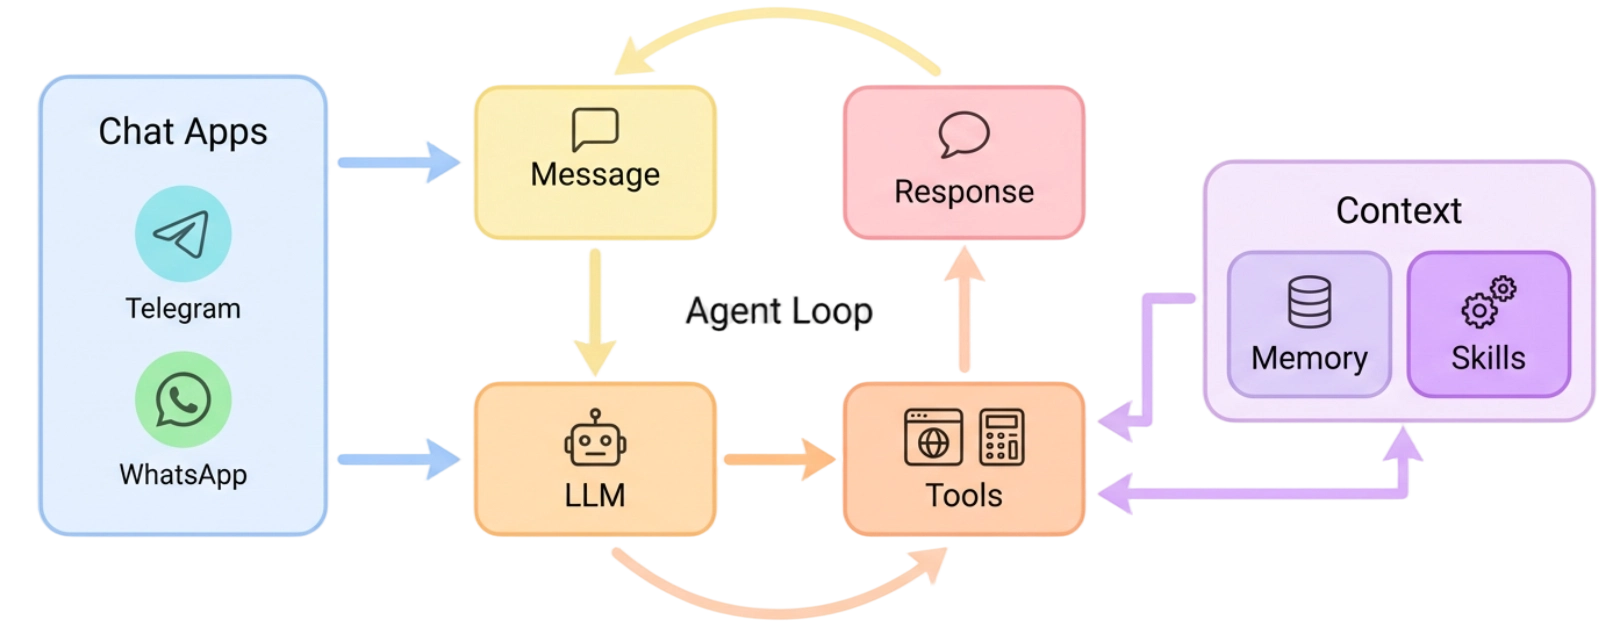
\includegraphics[width=0.85\textwidth]{figs/nanobot_arch.png}
    \caption{Esquema conceptual de la arquitectura del framework Nanobot.}
    \label{fig:NanobotArch}
\end{figure}

\subsubsection{API y comunicación}\label{subsec:agente-api-localmind}

El servidor de \gls{api} se evaluó de forma independiente al agente. Dentro del ecosistema de \gls{python}, Django REST Framework añade serialización y autenticación sobre \gls{django}, \Gls{fastapi} ofrece validación automática de datos con esquemas OpenAPI, y \Gls{flask} permite crear servicios mínimos \cite{djangorest2026,FastAPI,WelcomeFlaskFlask}. Sin embargo, la biblioteca \Gls{aiohttp} proporciona soporte asíncrono tanto para HTTP como para \gls{websocket} en un único bucle de eventos \cite{aiohttp2026}.

En cuanto a los protocolos, \Gls{websocket} permite mantener una conexión bidireccional continua, necesaria para transmitir en tiempo real (\emph{streaming}) las respuestas del modelo. Por su parte, el protocolo \Gls{rest} es idóneo para peticiones independientes y puntuales \cite{rfc6455,QueEsAPI}.

\textbf{Decisión.} Se utiliza \gls{aiohttp} para implementar el servidor. \Gls{websocket} es el canal principal para la respuesta en tiempo real, mientras que la \gls{api} \gls{rest} atiende las peticiones independientes. De este modo se aclara que el servidor no utiliza \gls{fastapi}.

\subsubsection{Instalador y configurador TUI}

La interfaz en terminal (\gls{tui}) de LocalMind guía al usuario en la detección del sistema, la elección del motor de inferencia, el modelo y las herramientas \gls{mcp}. Para su diseño se estudió como referencia el proyecto Gentle-AI, desarrollado en \gls{golang} con la biblioteca Bubble Tea y el patrón \gls{mvu} \cite{gentleai2026,bubbletea2026}, del que se tomaron ideas para la distribución visual, el uso del teclado y la navegación por pantallas.

\textbf{Decisión.} Se mantiene la \gls{tui} desarrollada en \gls{python} y se cita Gentle-AI como referencia de diseño e interfaz, sin que constituya una dependencia del código.

En la Figura~\ref{fig:TUIComparativa} se presenta la comparación visual entre la interfaz de terminal de Gentle-AI, en la Figura~\ref{fig:TUIGentle}, y la pantalla equivalente desarrollada en \gls{python} para LocalMind-AI, en la Figura~\ref{fig:TUILocalMind}.

\begin{figure}[h!tp]
    \centering
    \begin{subfigure}[b]{0.48\textwidth}
        \centering
        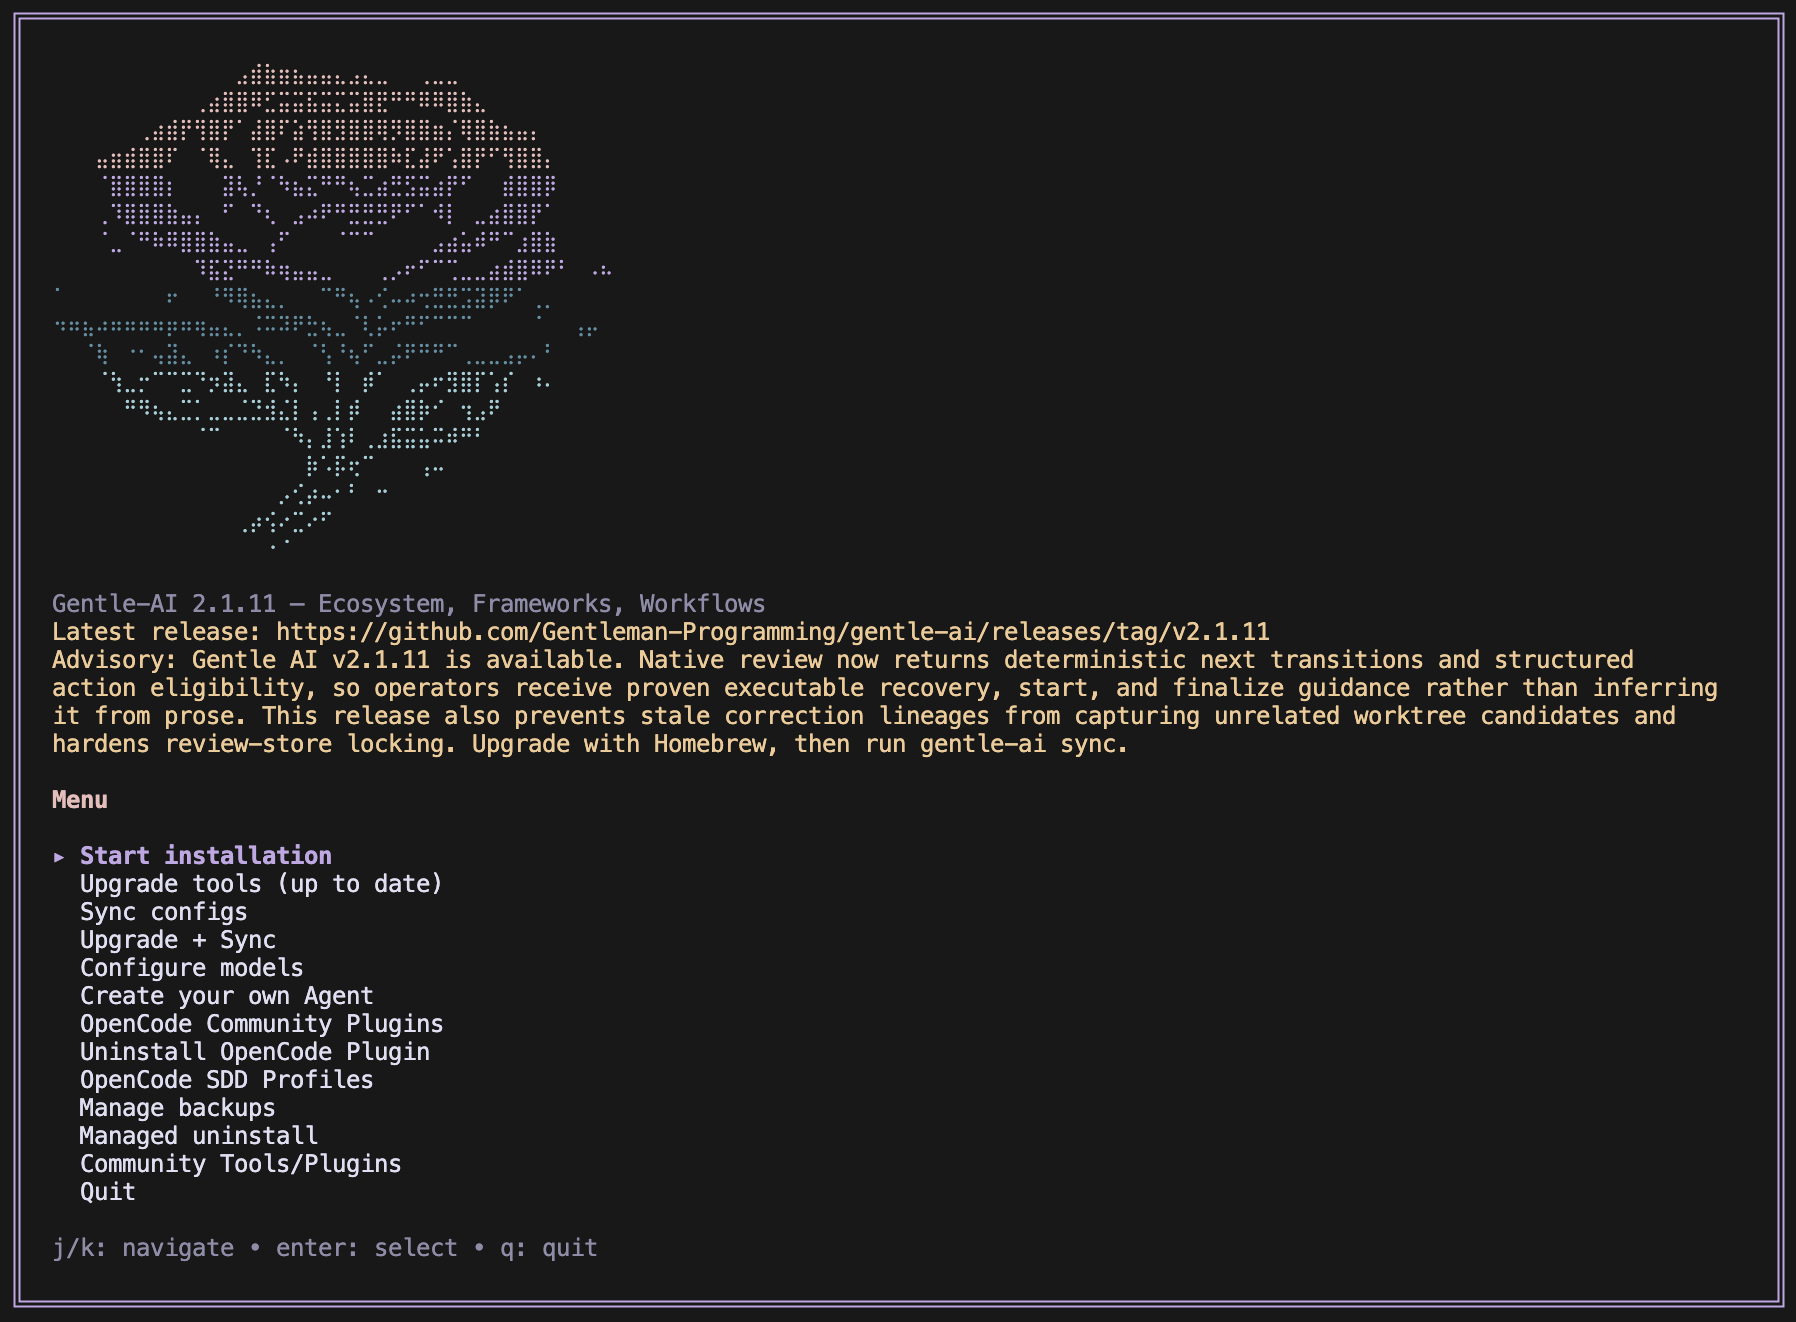
\includegraphics[width=\textwidth]{figs/tui_gentle-ai.png}
        \caption{Interfaz TUI de Gentle-AI en Golang \cite{gentleai2026}.}
        \label{fig:TUIGentle}
    \end{subfigure}
    \hfill
    \begin{subfigure}[b]{0.48\textwidth}
        \centering
        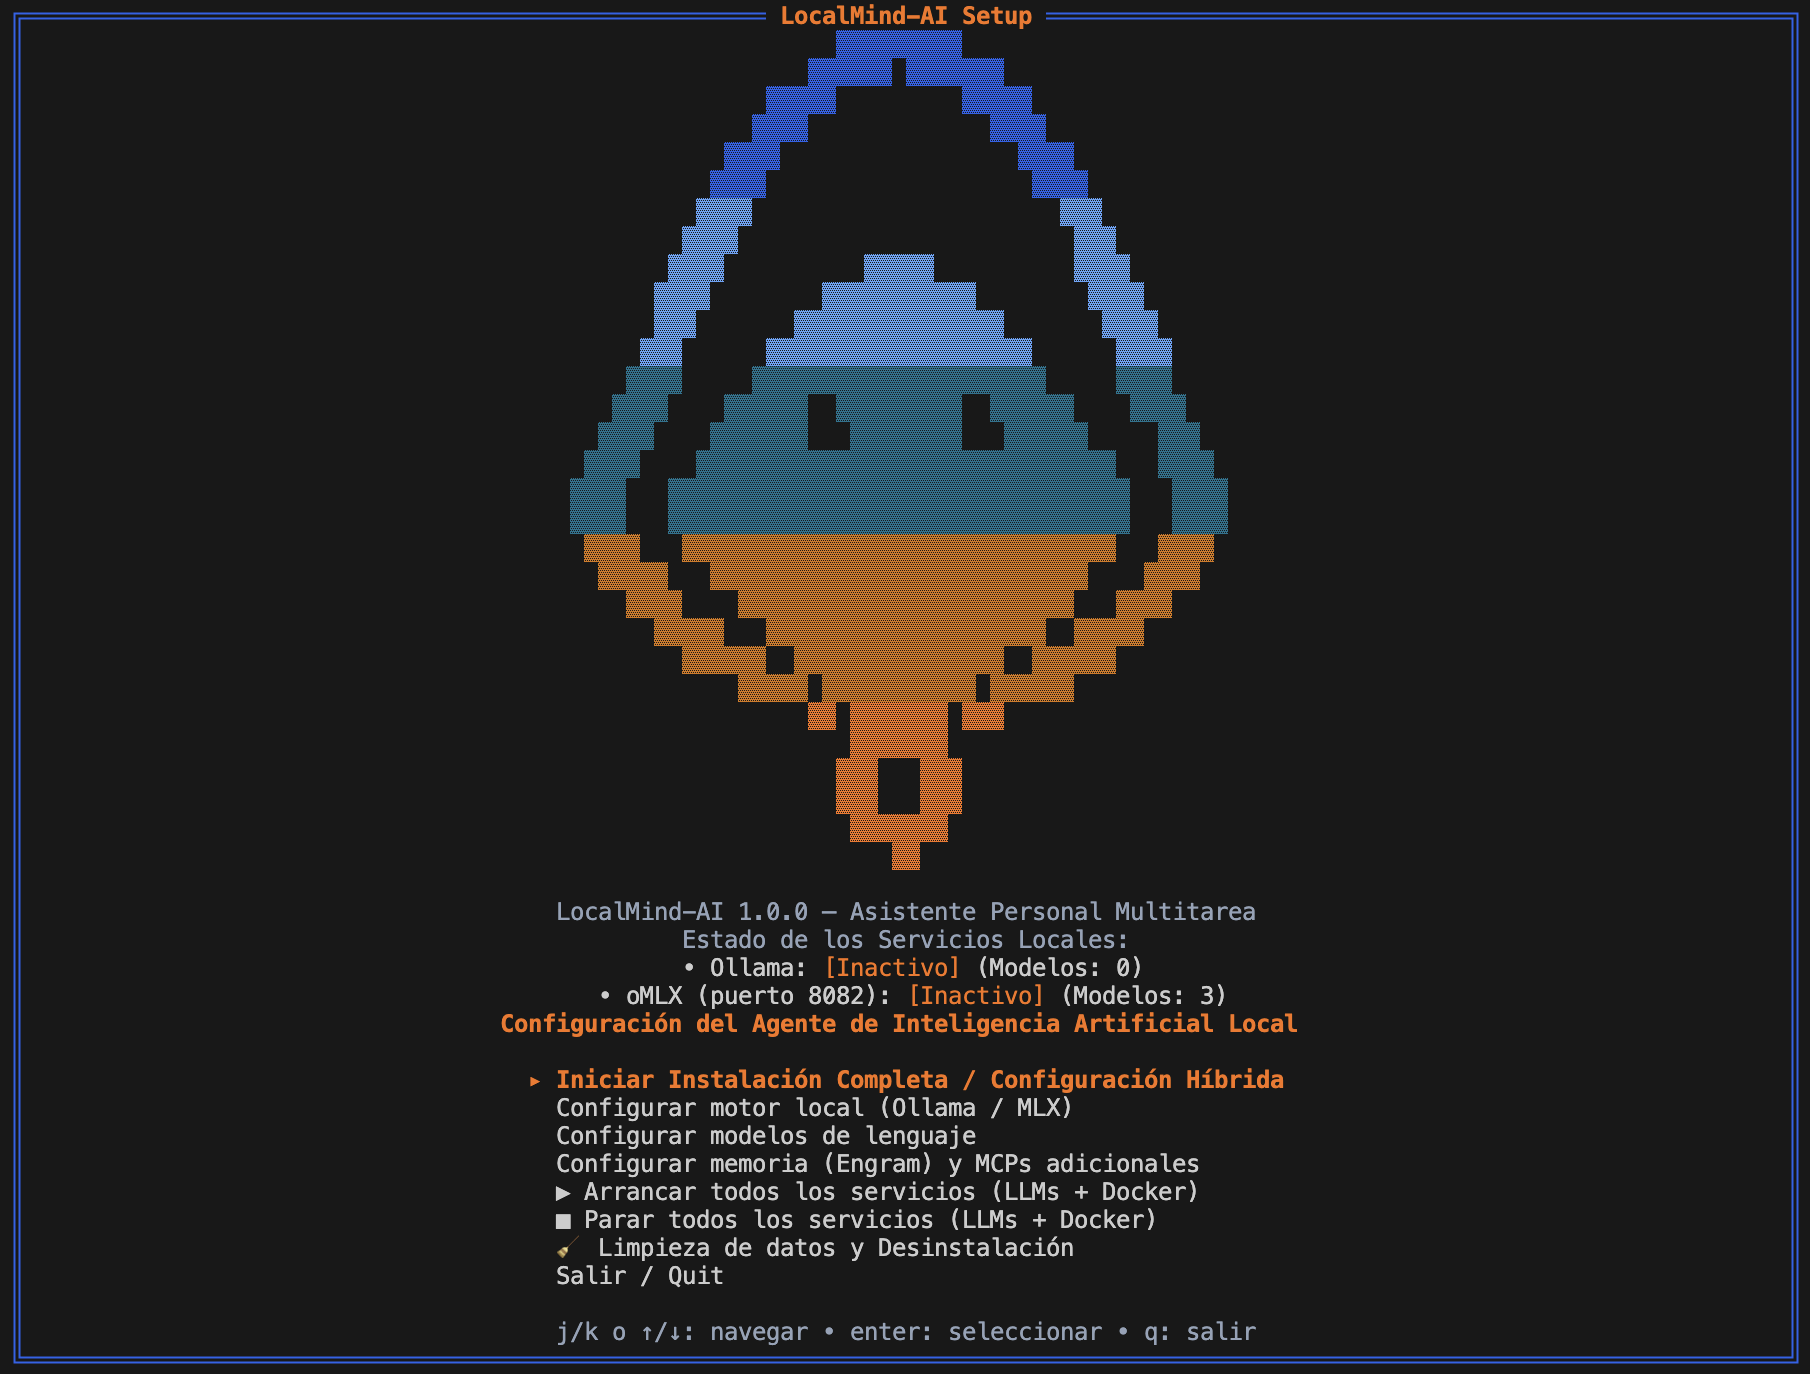
\includegraphics[width=\textwidth]{figs/tui_localmind-ai.png}
        \caption{Interfaz TUI de LocalMind-AI en Python.}
        \label{fig:TUILocalMind}
    \end{subfigure}
    \caption{Comparación visual entre la interfaz de terminal de Gentle-AI y la TUI de LocalMind-AI.}
    \label{fig:TUIComparativa}
\end{figure}

\subsubsection{Software de inferencia local}\label{subsec:inferencia-local-localmind}

Para la inferencia local se evaluaron varios motores. \Gls{ollama} simplifica la descarga y el uso de modelos mediante una \gls{api} local sencilla y está disponible en varios sistemas \cite{ollama2024}. El servidor \Gls{omlx} ofrece una \gls{api} compatible con OpenAI sobre \gls{mlx}, optimizada para Apple Silicon en \gls{macos} \cite{omlx2026}. El motor \Gls{vllm} está enfocado al alto rendimiento y procesamiento por lotes en servidores con muchos usuarios, unas ventajas poco relevantes para un asistente local individual \cite{vllm2026}. Por último, \Gls{chatrtx} combina inferencia y recuperación en \gls{windows} con tarjetas RTX, pero limita el sistema al ecosistema de NVIDIA \cite{nvidia2026chatrtx}.

\textbf{Decisión.} Se utiliza \gls{ollama} como motor general y \gls{omlx}/\gls{mlx} para entornos \gls{macos} con Apple Silicon. Ambos se ejecutan en el sistema anfitrión fuera de \gls{docker} para aprovechar la aceleración por \gls{hardware}.

\subsubsection{Modelos de IA generativa}

El sistema ofrece dos familias principales de modelos de 9.000 millones de parámetros, que son Ornith~1.0~9B y Qwen~3.5~9B, disponibles en versiones cuantizadas de 4 y 6 bits \cite{ornith9b4,ornith9b6,qwen359b}. La cuantización a 4 bits reduce el consumo de memoria y deja más recursos libres para el sistema, a costa de una pequeña pérdida de precisión. La de 6 bits conserva mejor la información de los pesos, pero requiere más \gls{ram} o \gls{vram}. La cuantización cambia la forma de representar los pesos, pero no altera el número de parámetros del modelo.

\textbf{Decisión.} La configuración recomendada en \gls{macos} es Ornith~1.0~9B cuantizado a 4 bits. Esta elección se documenta como la opción activa en las pruebas, si bien el usuario puede elegir entre Ornith/Qwen y cuantización de 4/6 bits según la memoria de su equipo.

En la Figura~\ref{fig:TUISelectorModelos} se ilustran las pantallas del instalador TUI de LocalMind-AI. La Figura~\ref{fig:TUITiposModelos} muestra la clasificación inicial de perfiles organizada en función del nivel de inteligencia y capacidad del modelo, mientras que la Figura~\ref{fig:TUIModelosCuantizacion} expone el catálogo de modelos específicos junto con la descripción comentada al lado de cada opción, la cual detalla la velocidad de respuesta esperada y el nivel de inteligencia estimado según los recursos disponibles del sistema.

\begin{figure}[h!tp]
    \centering
    \begin{subfigure}[b]{0.48\textwidth}
        \centering
        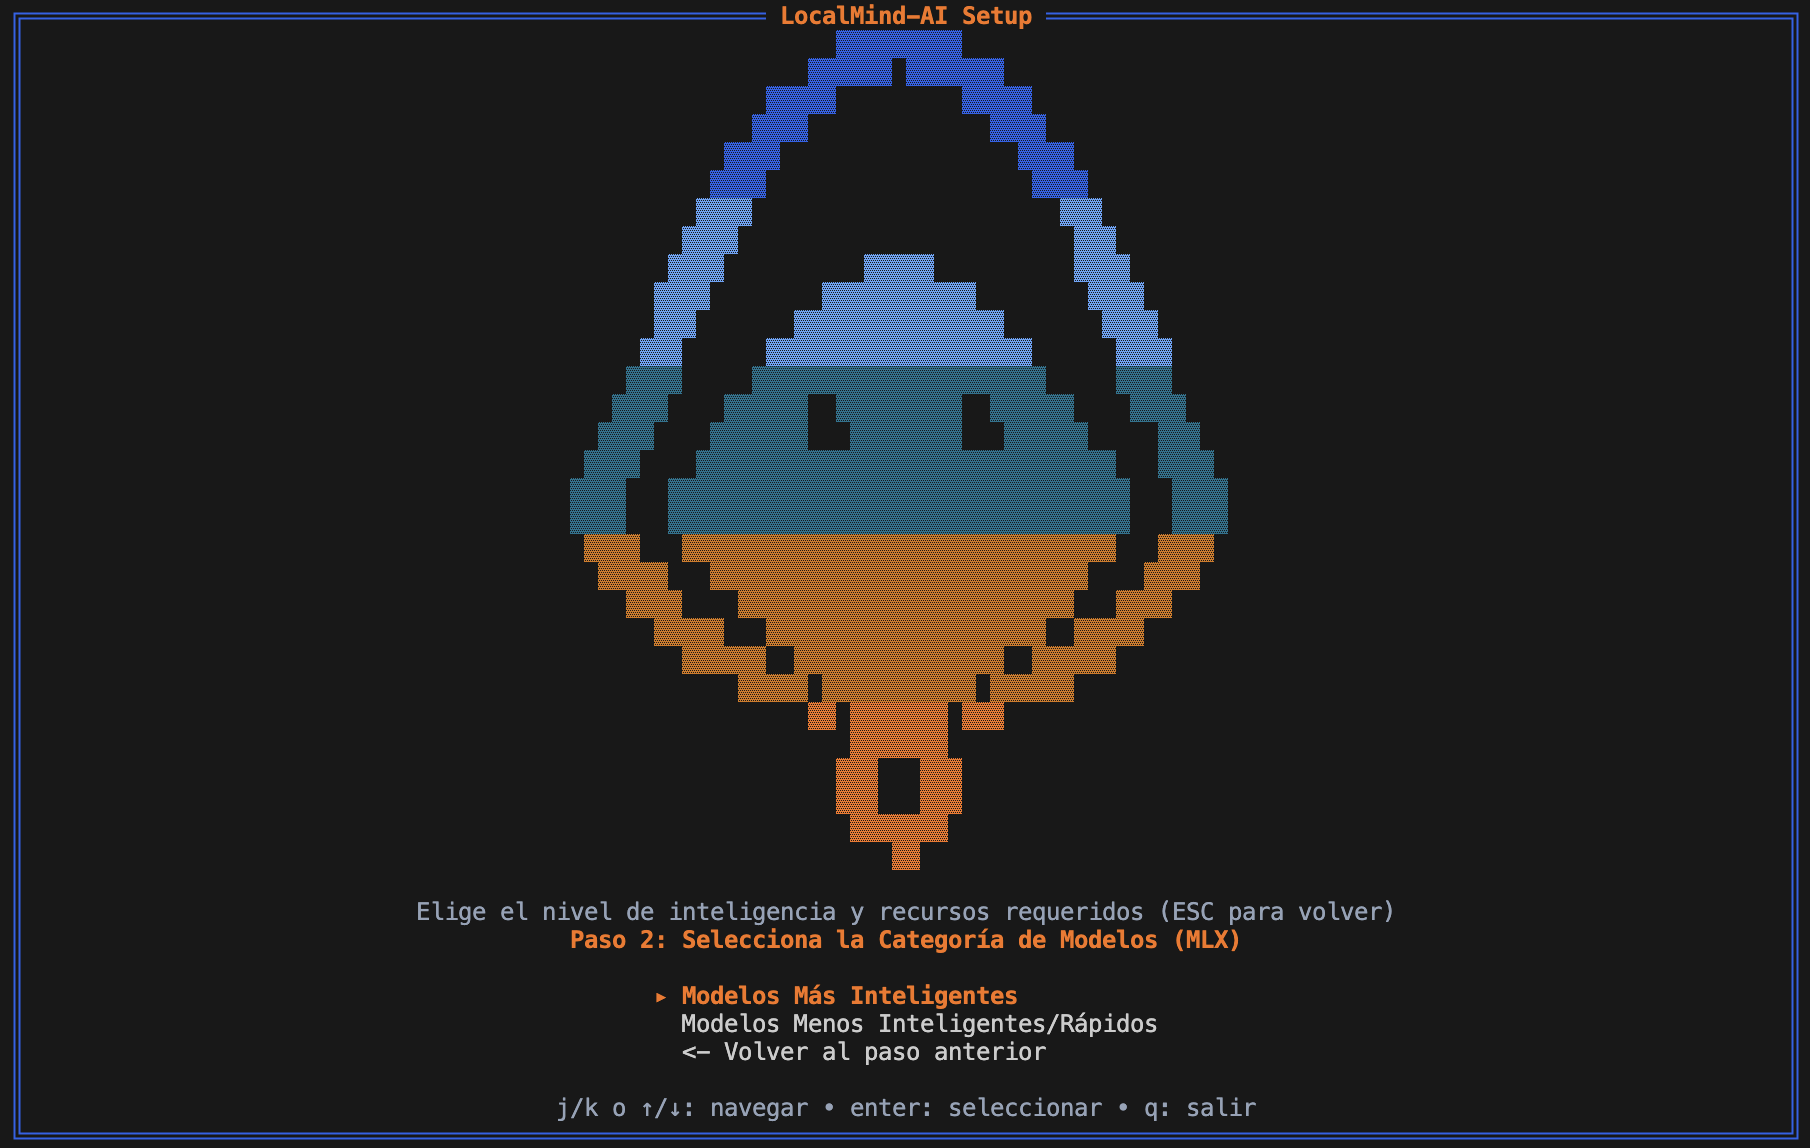
\includegraphics[width=\textwidth]{figs/selector-modelos-ia1.png}
        \caption{Selección por nivel de inteligencia y perfil del modelo.}
        \label{fig:TUITiposModelos}
    \end{subfigure}
    \hfill
    \begin{subfigure}[b]{0.48\textwidth}
        \centering
        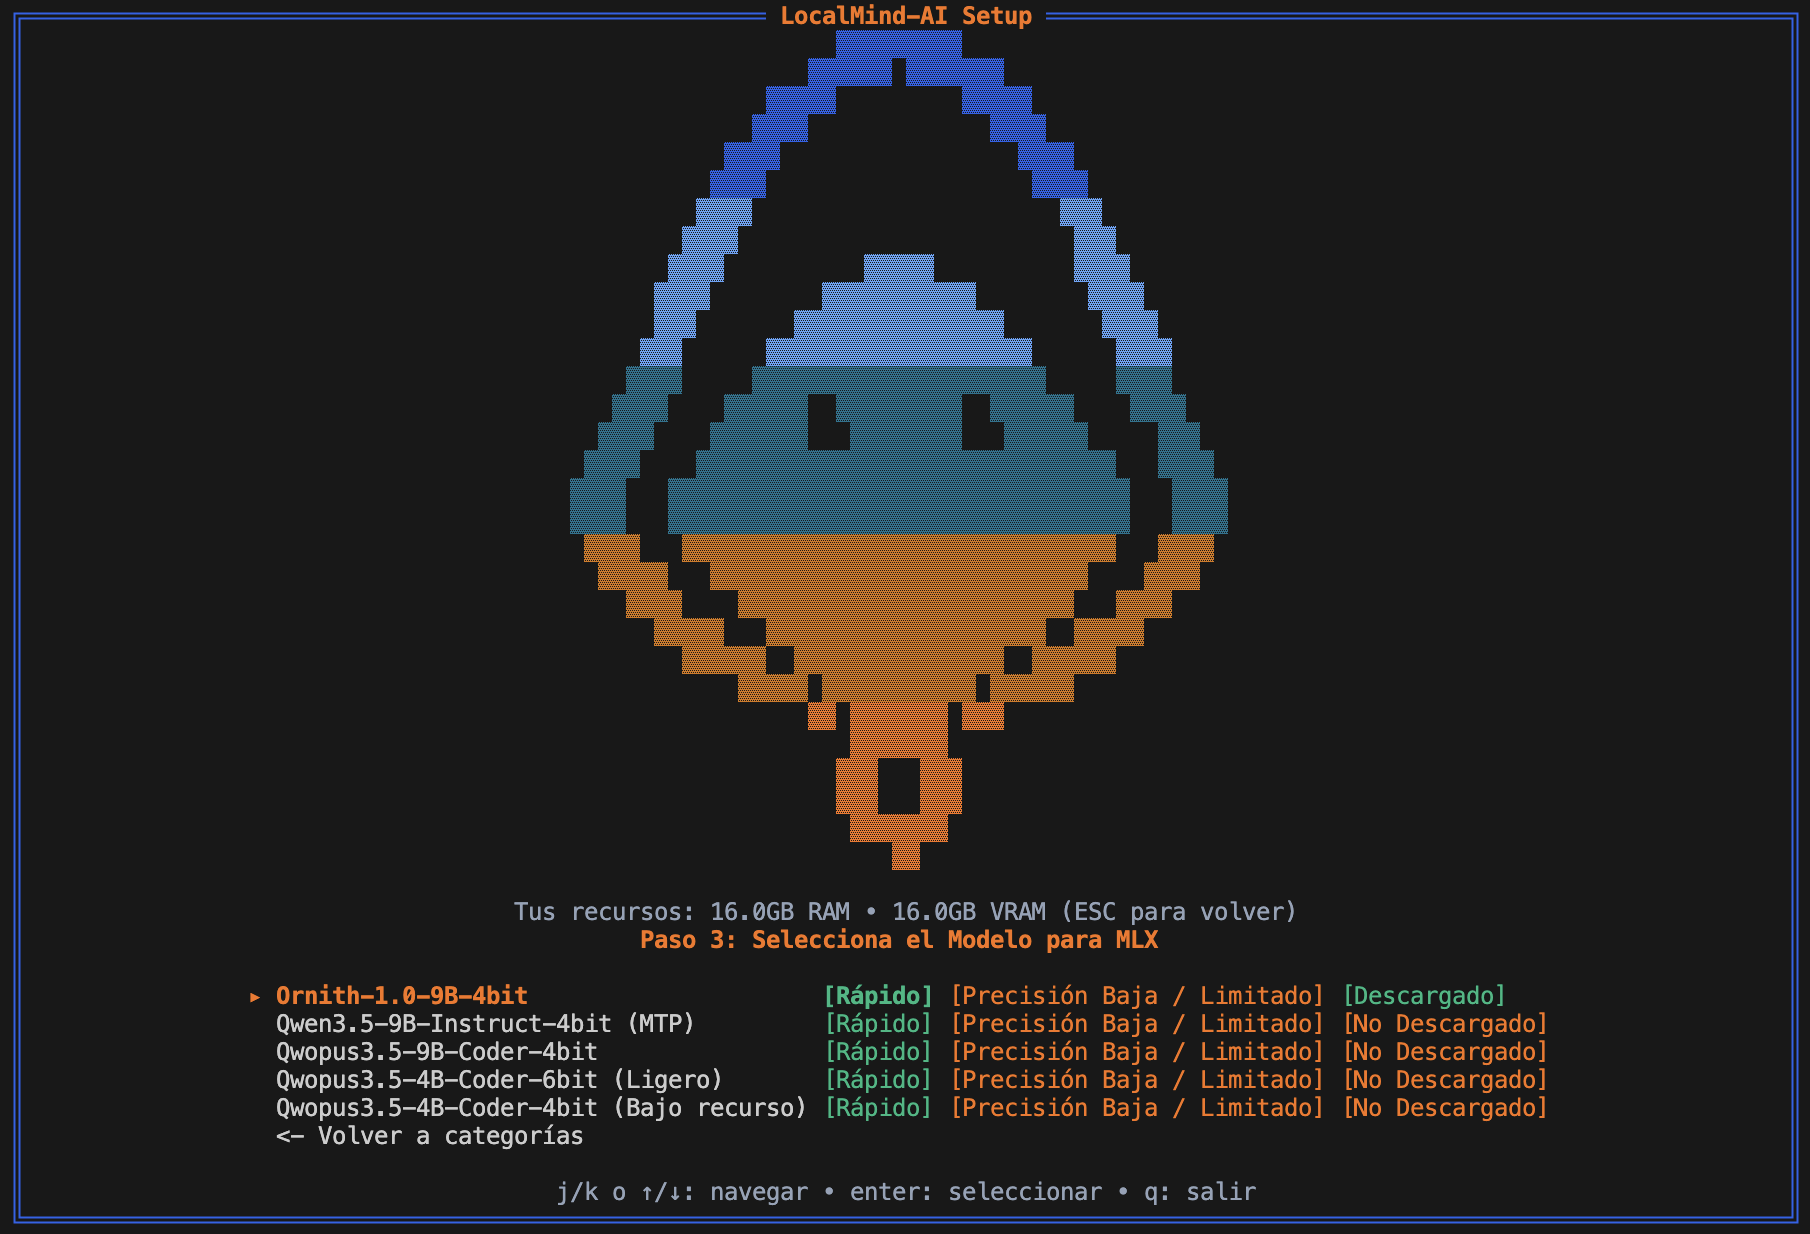
\includegraphics[width=\textwidth]{figs/selector-modelos-ia2.png}
        \caption{Catálogo de modelos con descripción y cuantización comentada.}
        \label{fig:TUIModelosCuantizacion}
    \end{subfigure}
    \caption{Pantallas del selector de modelos e inferencia en la TUI de LocalMind-AI.}
    \label{fig:TUISelectorModelos}
\end{figure}

\subsubsection{Recuperación, memoria y herramientas}\label{subsec:recuperacion-memoria-localmind}

Estos componentes cumplen funciones complementarias en el sistema. Para la base de datos vectorial, \Gls{chromadb} permite guardar documentos, incrustaciones y metadatos en una base de datos integrada, mientras que FAISS es una biblioteca de búsqueda y Qdrant requiere un servidor independiente \cite{chroma2026,faiss2026,qdrant2026}. Se elige \gls{chromadb} para no tener que administrar un servicio de base de datos adicional.

Para generar los \glspl{embeddings}, hacerlo en local garantiza la privacidad al no enviar documentos fuera del equipo. LocalMind utiliza el servicio de \glspl{embeddings} de \gls{ollama}, de modo que el proceso \gls{rag} mantiene esta dependencia incluso si el modelo conversacional se ejecuta con \gls{omlx} \cite{ollamaembeddings2026}.

Para ampliar las funciones del agente, el protocolo \gls{mcp} estandariza el uso de herramientas. Para guardar la conversación, los archivos \gls{jsonl} registran el historial de las sesiones, los ficheros \gls{markdown} guardan la memoria en un formato fácil de leer y el sistema \gls{engram} aporta búsqueda semántica sobre notas anteriores.

\textbf{Decisión.} Se combinan \gls{chromadb}, \glspl{embeddings} locales con \gls{ollama}, herramientas \gls{mcp}, sesiones en \gls{jsonl}, memoria en \gls{markdown} y \gls{engram}, manteniendo clara la función de cada elemento. El flujo de indexación y recuperación documental de LocalMind-AI sigue el esquema conceptual introducido en la Figura~\ref{fig:pipelineRag}, adaptando las fases de fragmentación, incrustación semántica y búsqueda por similitud vectorial a un entorno de ejecución íntegramente local.

En la Figura~\ref{fig:ListadoHerramientasMCP} se expone la pantalla de la TUI de LocalMind-AI correspondiente al listado de herramientas \gls{mcp} registradas y disponibles para el agente.

\begin{figure}[h!tp]
    \centering
    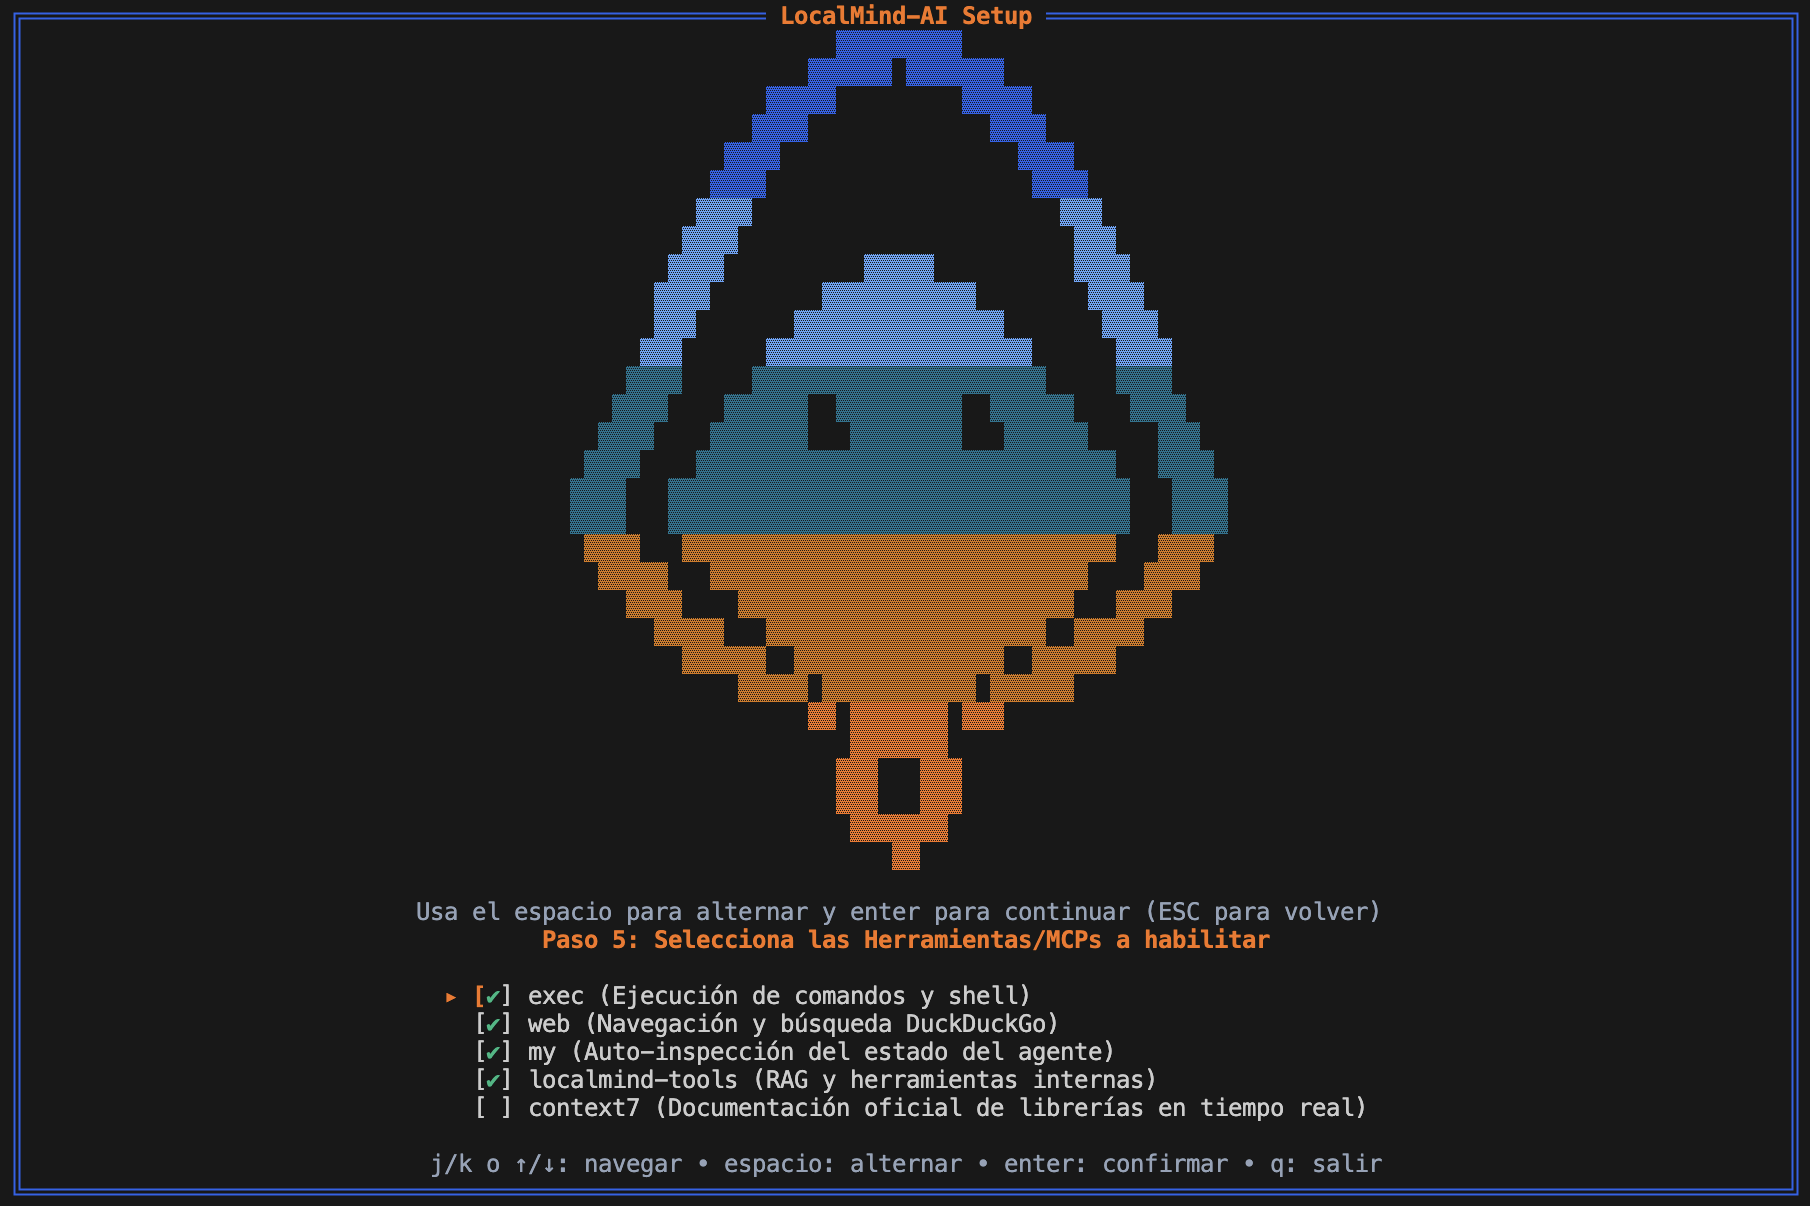
\includegraphics[width=0.82\textwidth]{figs/listado-herramientas-localmind.png}
    \caption{Listado de herramientas MCP integradas y disponibles en la TUI de LocalMind-AI.}
    \label{fig:ListadoHerramientasMCP}
\end{figure}

\subsection{Entorno de desarrollo, gestión de versiones y diseño de diagramas}\label{subsec:entorno-calidad-localmind}

La memoria se redacta en \gls{latex} con Visual Studio Code y se compila localmente con \gls{mactex}. La herramienta Arara automatiza el proceso con pdfLaTeX, Biber y las pasadas necesarias para referencias y glosarios \cite{LaTeXDocumentPreparation,VisualStudioCode,mactex2026,IslandoftexArara2025}, permitiendo trabajar sin depender de un editor web. En la Figura~\ref{fig:visual-mactex-compiler} se observa la interfaz del entorno de desarrollo integrado Visual Studio Code junto con el flujo de compilación local y las herramientas auxiliares empleadas para construir el documento.

Las referencias bibliográficas se gestionan con Zotero, mientras que BibLaTeX y Biber procesan el archivo \texttt{references.bib} durante la compilación \cite{ZoteroYourPersonal,biber2026}. El control de versiones se realiza con Git y GitHub como repositorio remoto \cite{git2026,GitHubcomDocumentacionAyuda}. Asimismo, Visual Studio Code se utiliza para escribir el código en Python, JavaScript, Shell, YAML y los diagramas.

Para la creación de diagramas se utilizan Visual Paradigm, Mermaid y PlantUML \cite{IdealModelingDiagramming,Mermaid,plantuml2026}, elaborando el diagrama de Gantt del proyecto únicamente con PlantUML.

\textbf{Decisión.} El entorno de desarrollo está formado por Visual Studio Code, LaTeX, MacTeX, Arara, Zotero, Biber, Git, GitHub, Visual Paradigm, Mermaid y PlantUML. Cada herramienta se selecciona por su utilidad práctica dentro del proyecto.

\begin{figure}[h!tp]
    \centering
    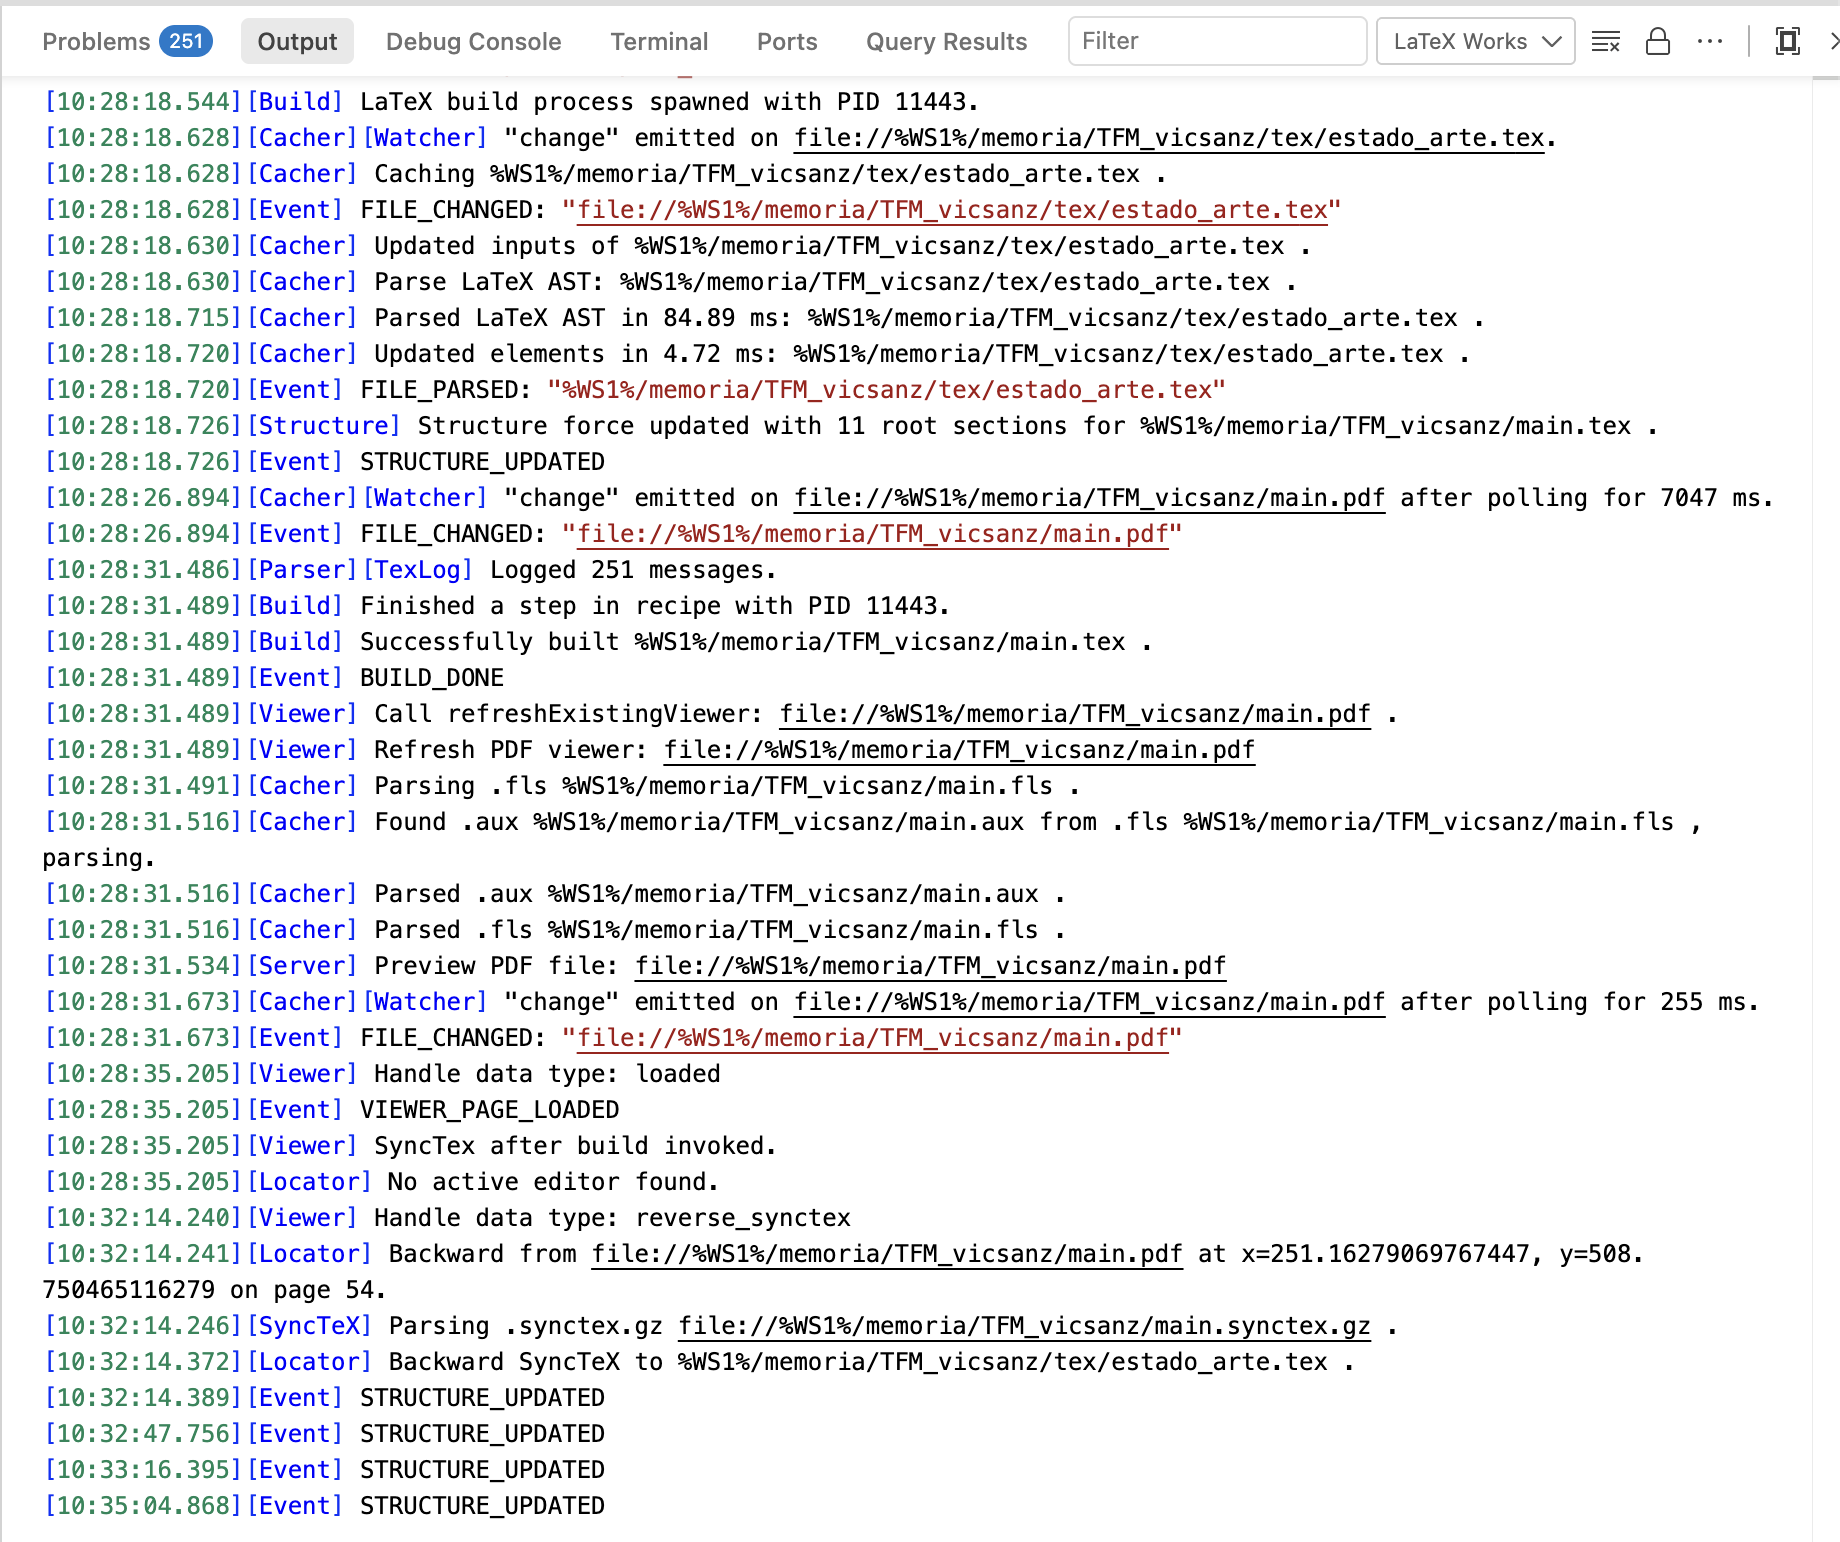
\includegraphics[width=0.80\textwidth]{figs/visual_mactex_compiler.png}
    \caption{Entorno de desarrollo empleado para compilar la memoria.}
    \label{fig:visual-mactex-compiler}
\end{figure}

\subsection{Conclusiones}\label{subsec:conclusiones-evaluacion-localmind}

La evaluación de tecnologías define una arquitectura modular y práctica. Docker Compose separa el agente y el cliente web en dos servicios: \gls{nanobot} concentra la comunicación y las herramientas, mientras que \gls{nginx} sirve los activos estáticos exportados por \gls{expo}. El navegador se comunica directamente con el agente mediante \gls{websocket} y \gls{rest}, y los modelos se procesan en el sistema anfitrión para aprovechar su aceleración. La memoria y el almacenamiento, por su parte, se dividen en componentes específicos. En la Tabla~\ref{tab:tecnologias-localmind} se resumen las decisiones tecnológicas adoptadas en el proyecto.

\begin{sidewaystable}[h!tp]
    \centering
    \scriptsize
    \setlength{\tabcolsep}{5pt}
    \renewcommand{\arraystretch}{1.12}
    \begin{tabularx}{\textwidth}{|>{\raggedright\arraybackslash}p{3.1cm}|>{\raggedright\arraybackslash}p{5.1cm}|>{\raggedright\arraybackslash}X|}
        \hline
        \textbf{Tipo}                    & \textbf{Necesidad}        & \textbf{Componente}                                                                                             \\
        \hline
        \multirow{2}{=}{Hardware}        & Portátiles de validación  & MSI Pulse GL66 12UEK-085ES y MacBook Air M4                                                                     \\
        \cline{2-3}
                                         & Referencia descartada     & HP OMEN 15-ce033ns, insuficiente para la validación prevista                                                    \\
        \hline
        \multirow{4}{=}{Infraestructura} & Sistemas anfitriones      & \Gls{windows}, \gls{macos} y compatibilidad \gls{linux}                                                         \\
        \cline{2-3}
                                         & Contenedores              & \Gls{docker}                                                                                                    \\
        \cline{2-3}
                                         & Despliegue reproducible   & \Gls{dockercompose} con servicios \texttt{nanobot} y \texttt{frontend}; \gls{mcp}/\gls{engram} como subprocesos \\
        \cline{2-3}
                                         & Aceleración               & \Gls{ollama} u \gls{omlx}/\gls{mlx} ejecutados nativamente en el host                                           \\
        \hline
        \multirow{12}{=}{Software}       & Lenguajes del producto    & \Gls{python}, \gls{javascript}, Shell/\gls{bash} y \gls{yaml}                                                   \\
        \cline{2-3}
                                         & Cliente web               & \Gls{reactnative} Web con \gls{expo}, exportado y servido por \gls{nginx}                                       \\
        \cline{2-3}
                                         & Núcleo del agente         & \Gls{nanobot}                                                                                                   \\
        \cline{2-3}
                                         & API y comunicación        & \gls{aiohttp}, \gls{websocket} y \gls{rest}                                                                     \\
        \cline{2-3}
                                         & Instalador/configurador   & \Gls{tui} \gls{python} con \gls{ansi}, inspirada en Gentle-AI                                                   \\
        \cline{2-3}
                                         & Inferencia local          & \Gls{ollama} y \gls{omlx}/\gls{mlx}                                                                             \\
        \cline{2-3}
                                         & Modelos                   & Ornith 1.0 9B y Qwen 3.5 9B, cuantizaciones de 4/6 bits                                                         \\
        \cline{2-3}
                                         & Recuperación documental   & \Gls{chromadb} y \glspl{embeddings} locales mediante \gls{ollama}                                               \\
        \cline{2-3}
                                         & Herramientas y memoria    & \Gls{mcp}, \gls{engram}, \gls{jsonl} y \gls{markdown}                                                           \\
        \cline{2-3}
                                         & Memoria y referencias     & LaTeX, MacTeX, Arara, Zotero y Biber                                                                            \\
        \cline{2-3}
                                         & Versionado y desarrollo   & Git, GitHub y Visual Studio Code                                                                                \\
        \cline{2-3}
                                         & Diagramas y planificación & Visual Paradigm, Mermaid y PlantUML, Gantt con PlantUML                                                         \\
        \hline
    \end{tabularx}
    \caption{Tecnologías seleccionadas para el desarrollo y la validación de LocalMind-AI.}
    \label{tab:tecnologias-localmind}
\end{sidewaystable}
